\documentclass[a4paper,12pt]{article}
\setcounter{secnumdepth}{2}
\newcommand{\code}[1]{{\footnotesize{{\tt #1}}}}
\usepackage{natbib}
\usepackage{color}
\usepackage{graphicx}
\usepackage{listings}
\lstset{
basicstyle=\small\ttfamily,
columns=flexible,
breaklines=true
}
\addtolength{\textwidth}{2cm} % a = -2b, where this is a and below is b
\addtolength{\hoffset}{-1cm}
\addtolength{\textheight}{2cm} % c = -d, where this is c and d is below
\addtolength{\voffset}{-2cm}
\begin{document}
\title{EMIM: Estimation of Maternal, Imprinting and interaction effects using Multinomial modelling}
\date{}
\author{}
\maketitle
\newpage
\tableofcontents
\newpage
\section{Introduction}
\label{introduction}

According to Wikipedia, ``Emim'' was the Moabite name for one of the tribes of Rephaim. They are described in Deuteronomy chapter 2 as having been a powerful people, populous and having a successful kingdom. The Emim are also mentioned in Genesis 14:5 where the name is translated as ``the dreaded ones''. 

Hopefully our program EMIM will prove an equally powerful tool for the detection of complex effects in genetic disease studies... 
\subsection{Program information and citation}
\label{information}

If you use the PREMIM/EMIM software in your work then please reference the accompanying software manuscript \citet{howey:cordell:12}: 
\vspace{0.35cm} \begin{lstlisting}

@article{howey:cordell:12,
  author = {Howey, R and Cordell, H J},
  title = {{PREMIM} and {EMIM}: Tools for estimation of maternal, imprinting and interaction effects using multinomial modelling},
  journal = {{BMC} Bioinformatics},
  volume = {13},
  pages = {149},
  year = {2012}
}              

\end{lstlisting} \vspace{0.35cm}
For use of the methodology of the multinomial likelihood approach used by this program, please reference the accompanying manuscript \citet{ainsworth:etal:11}: 
\vspace{0.35cm} \begin{lstlisting}

@article{ainsworth:etal:11,
  author={Ainsworth, H F and Unwin, J and Jamison, D L and Cordell, H J},
  title = {Investigation of maternal effects, maternal-foetal interactions and parent-of-origin effects (imprinting), using mothers and their offspring},
  journal = {Genet Epidemiol},
  volume = {35},
  pages = {19-45},
  number = {1},
  month = {January},
  year = {2011}
}

\end{lstlisting} \vspace{0.35cm}
You are STRONGLY recommended to read this paper before using EMIM in order to understand the notation and parameter restrictions/analysis options used. 

If you have used PREMIM/EMIM to estimate parent-of-origin effects with the use of SHAPEIT2 to estimate the parent-of-origin of alleles, please reference \citet{howey:etal:15}: 
\vspace{0.35cm} \begin{lstlisting}

@article{howey:etal:15,
author={Howey, R and Mamasoula, C and T\"opf, A and Nudel, R and Goodship, J A and Keavney, B D and Cordell, H J},
title={Increased Power for Detection of Parent-of-Origin Effects via the Use of Haplotype Estimation},
journal={The American Journal of Human Genetics},
volume={97},
number={3},
pages={419-434},
year={2015}
}

\end{lstlisting} \vspace{0.35cm}
EMIM is a FORTRAN 77 program with some FORTRAN 90 features and compiles under Linux or Windows (DOS) using a suitable compiler e.g. gfortran. We have not tried compiling on any other system, but see no reason why the program should not compile provided an appropriate FORTRAN compiler is available. To run EMIM under Windows, you will need to use the command line interface (i.e. open a command line (DOS) window). 

EMIM uses a maximisation subroutine MAXFUN that was originally written as part of (a former early version of) the S.A.G.E. package: \\ http://darwin.cwru.edu/sage/

Users of S.A.G.E are asked to insert the following acknowledgment in any publication that uses results obtained from S.A.G.E.: 

``(Some of) The results of this paper were obtained by using the program package S.A.G.E., which is supported by a U.S. Public Health Service Resource Grant (RR03655) from the National Center for Research Resources'' (it is important that the grant number appears under ``acknowledgments''). 

Please see more details on the S.A.G.E website: \\ http://darwin.cwru.edu/sage/?q=node/5

Copyright, 2012-2016 Heather Cordell and Richard Howey, GNU General Public License, version 3. 

%============ End of subsection "information"============


%================== End of section "introduction"==================

\section{Quick Start}
\label{quick-start}
\begin{enumerate}

\item Download set of executable files for EMIM (includes PREMIM) for your required platform: 
{\begin{center}\begin{tabular}{ll}
Platform  & File\\
\hline
Linux (x86\_64) & emim-v3.22-linux-x86\_64.zip\\
Linux (x86\_32) & emim-v3.22-linux-x86\_32.zip\\
Windows (x86\_64) & emim-v3.22-windows-x86\_64.zip\\
Windows (x86\_32) & emim-v3.22-windows-x86\_32.zip\\
\end{tabular}\end{center}}
and unzip the set of files into a directory. 
\item Run PREMIM on your pedigree data: \vspace{0.35cm} \begin{lstlisting}
./premim mydatafile.ped 
\end{lstlisting} \vspace{0.35cm}where mydatafile.ped is a PLINK text pedigree file, or alternatively a better (faster) option is to use a PLINK binary pedigree file (.bed): \vspace{0.35cm} \begin{lstlisting}
./premim mydatafile.bed 
\end{lstlisting} \vspace{0.35cm}(These commands will assume the existence of either a corresponding .map file or corresponding .fam and .bim files.) 
\item Run EMIM in the same directory as the .dat files created by PREMIM: \vspace{0.35cm} \begin{lstlisting}
./emim 
\end{lstlisting} \vspace{0.35cm}
\item Check the results of EMIM in the files: {\it emimresults.out} and {\it emimsummary.out}. 
\item Do another analysis by changing the parameters given to EMIM by editing the parameter file {\it emimparams.dat}.\end{enumerate}

For more details and advanced options on PREMIM please read  section \ref{premim}, and on EMIM please read  section \ref{emim}. 

If a suitable executable file is not available for your system then you should download and compile the source code as explained in  section \ref{comp}. 

%================== End of section "quick-start"==================

\section{Slow Start}
\label{comp}

If you have successfully downloaded executable files for PREMIM and EMIM that work on your system then you may skip this section. However, if you need to compile the source codefor your system then please follow the instructions below. 
\subsection{Compilation of PREMIM source code}
\label{comp-premim}

The source code for PREMIM is written in C++ and can be compiled on any system with a C++ compiler installed. The code can be compiled by typing something similar to: 
\vspace{0.35cm} \begin{lstlisting}
g++ *.cpp -o premim 
\end{lstlisting} \vspace{0.35cm}
Also, if you are using the GNU compiler it is often a good idea to use the -O3 option to optimize the code for faster execution: 
\vspace{0.35cm} \begin{lstlisting}
g++ -O3 *.cpp -o premim 
\end{lstlisting} \vspace{0.35cm}
If you wish to use gzipped files with PREMIM then you may do so by installing the following two libraries: 

{\begin{center}\begin{tabular}{ll}
Library  & Website\\
\hline
zlib  & http://www.zlib.net/\\
gzstream  & http://www.cs.unc.edu/Research/compgeom/gzstream/\\
\end{tabular}\end{center}}

Then it is necessary to uncomment the following line in the \code{main.h} file: 
\vspace{0.35cm} \begin{lstlisting}
//#define USING_GZIP 
\end{lstlisting} \vspace{0.35cm}
to become 
\vspace{0.35cm} \begin{lstlisting}
#define USING_GZIP 
\end{lstlisting} \vspace{0.35cm}
Once the libraries are installed and the above line uncommented PREMIM can be compiled by typing something similar to: 
\vspace{0.35cm} \begin{lstlisting}
g++ -O3 *.cpp -o premim -I/home/username/gzstream/gzstream
 -L/home/username/gzstream/gzstream
 -L/home/username/zlib/zlib-1.2.5 -lgzstream -lz

\end{lstlisting} \vspace{0.35cm}
%============ End of subsection "comp-premim"============

\subsection{Compilation of EMIM source code}
\label{comp-emim}

EMIM is written in Fortran 77 with some Fortran 90 features. Compile the program under Unix, Linux or Windows using: 
\vspace{0.35cm} \begin{lstlisting}

gfortran emim.f maxfun.f -o emim

\end{lstlisting} \vspace{0.35cm}
This should produce an executable that can by run by typing \code{./emim} (or else by giving the full pathname e.g. \code{/home/username/EMIM-v2.05/emim}) 

Some compilers may produce a number of warning messages when compiling EMIM. Provided that an executable file \code{emim} has been created, we do not anticipate that you need to be too concerned about these warnings. 

A set of example input files is included in the EMIM distribution. These example files are not intended to be particularly realistic but simply can be used to check that the program runs. 

%============ End of subsection "comp-emim"============


%================== End of section "comp"==================

\section{PREMIM: Pedigree file conversion}
\label{premim}

The program EMIM requires a number of input files as described in  section \ref{emim}; the program PREMIM is written as a useful tool to create these files from standard format pedigree files. Basic usage of the program is given by typing: 
\vspace{0.35cm} \begin{lstlisting}

./premim data.ped

\end{lstlisting} \vspace{0.35cm}
where {\it data.ped} is a PLINK pedigree file with corresponding MAP file, {\it data.map}, in the same directory. Alternatively, you can use a PLINK binary pedigree file: 
\vspace{0.35cm} \begin{lstlisting}

./premim data.bed

\end{lstlisting} \vspace{0.35cm}
where {\it data.bed} is a PLINK binary pedigree file with corresponding files, {\it data.bim} and {\it data.fam}, in the same directory. 

PREMIM will produce a number of output files (ready for subsequent input to EMIM) and a copy of the screen output is written to the file {\it premim.log} 

{\bf Note that PREMIM and EMIM are designed for the analysis of diallelic autosomal loci (i.e. SNPs on chromosomes 1-22) only.} 

If your input files contain SNPs on any chromosomes other than 1-22, PREMIM will exit with a warning message and will not produce any output files (apart from {\it premim.log}). We suggest you use PLINK to remove any SNPs on chromosomes other than 1-22 {\bf prior} to embarking on an analysis with PEMIM and EMIM. 
\subsection{Usage}
\label{premim-usage}

There are several different options available on how to run PREMIM from the command line. Full usage of the program is given by: 
\vspace{0.35cm} \begin{lstlisting}

./premim [options] datafile [mapfile]

\end{lstlisting} \vspace{0.35cm}
where \code{options} are given by a number of optional switches; the \code{datafile} is a pedigree file given either as a PLINK pedigree file (.ped), a gzipped PLINK pedigree file (.gzip), or a PLINK binary pedigree file (.bed). PREMIM will look for a corresponding .map file or .bim and .fam files in the same directory. Alternatively, if you are using a non-binary PLINK pedigree file, you can specify an alternatively-named non-binary \code{mapfile} (where the SNPs must appear in the same order as in the pedigree file). 
\subsubsection{Options}
\label{premim-options}

The available options are summarised below: 

{\begin{center}\begin{tabular}{ll}
Option  & Description\\
\hline
-a  & estimate SNP allele frequencies (and output to \code{emimmarkers.dat})\\
-s n dir  & split SNP output into groups of size n in directory dir\\
-n name  & add a name to the end of the output files\\
-so  & suppress output to screen\\
-xa  & allow extra affected case trios per pedigree (not permitted with -ihap,  section \ref{poo}) \\
-xu  & allow extra unaffected control matings per pedigree\\
-pb file  & use a proband file, listing affected subjects of interest\\
-rmaj  & use major allele as risk allele (denoted as allele ``2'' in EMIM)\\
-rout file  & output a listing of the risk alleles (and the SNP names and numbers) to file\\
-rfile file  & use the alleles in file as risk alleles\\
-cg  & child genotype\\
-ct  & child trend (default)\\
-mg  & mother genotype\\
-mt  & mother trend\\
-im  & imprinting, maternal\\
-ip  & imprinting, paternal\\
-imw  & imprinting, maternal (Weinberg 1999 parameterisation)\\
-ipw  & imprinting, paternal (Weinberg 1999 parameterisation)\\
\end{tabular}\end{center}}

%====== End of subsubsection "premim-options"======


%============ End of subsection "premim-usage"============

\subsection{Input files}
\label{premim-input}

There are three different ways to supply the pedigree data to PREMIM: 
\begin{enumerate}

\item {\bf .ped} and {\bf .map}. A PLINK pedigree file (.ped) and a MAP file (.map). It is not necessary to specify the MAP file - this will be assumed to be in the same location as the .ped file. For example typing: \vspace{0.35cm} \begin{lstlisting}

./premim mydata.ped

\end{lstlisting} \vspace{0.35cm}will assume that {\it mydata.map} exists in the same location as {\it mydata.ped}. If it does not exist PREMIM will stop and report that the file cannot be found. If one wishes to specify a different .map file, say {\it mymapfile.map}, then this may be done by typing: \vspace{0.35cm} \begin{lstlisting}

./premim mydata.ped mymapfile.map

\end{lstlisting} \vspace{0.35cm}
\item {\bf .bed, .fam} and {\bf .bim}. A PLINK binary pedigree file (.bed) together with the corresponding family information file (.fam) and the extended MAP file (.bim). These three files can be created in PLINK in order to compress pedigree information. To use PREMIM with a .bed file, say {\it mydata.bed}, simply type: \vspace{0.35cm} \begin{lstlisting}

./premim mydata.bed

\end{lstlisting} \vspace{0.35cm}The .fam and .bim files will be assumed to exist in the same directory as the .bed file with names {\it mydata.fam} and {\it mydata.bim} respectively. If these files do not exist PREMIM will stop and report this. 
\item {\bf .gzip} and {\bf .map}. A gzipped pedigree file (.gzip) and a MAP file (.map). Another way to compress pedigree files is to create a .gzip file - these files may be used directly in PREMIM without the need to unzip the files. The MAP file (.map) file should not be gzipped and can be specified or assumed (similarly to when using a .ped file).\end{enumerate}

{\bf Note:} if you wish to use multiple pedigree files it is recommended that you use PLINK to combine these files into one file, this can then be used as input into PREMIM. 

%============ End of subsection "premim-input"============

\subsection{Output files}
\label{premim-output}

The program PREMIM outputs the following files: 
\begin{enumerate}

\item {\bf {\it caseparenttrios.dat}, {\it casemotherduos.dat}, {\it casefatherduos.dat}, {\it caseparents.dat}, {\it casemothers.dat}, {\it casefathers.dat}, {\it cases.dat}, {\it conparents.dat}, {\it conmotherduos.dat}, {\it confatherduos.dat}} and {\bf {\it cons.dat}}. These files contain the different counted genotype combinations for every SNP and every pedigree. 
\item {\bf {\it emimparams.dat}}. This file contains the required parameter settings for EMIM and is described in  section \ref{emimparams}. This file is created with a set of default values which may be changed as appropriate for the type of analysis that you wish to perform. There are a number of options that can be given to PREMIM to set the initial options created in this file. The following options choose the kind of child analysis (i.e. the way in which you wish to model child genotype or allele effects): \begin{itemize}

\item {\bf -cg}. Perform a child genotype analysis. 
\item {\bf -ct}. Perform a child trend analysis (allele effects).\end{itemize}
The following options choose the kind of mother analysis: \begin{itemize}

\item {\bf -mg}. Perform a mother genotype analysis. 
\item {\bf -mt}. Perform a mother trend analysis (maternal allele effects).\end{itemize}
The following options choose the kind of imprinting analysis: \begin{itemize}

\item {\bf -im}. Perform a maternal imprinting analysis. 
\item {\bf -ip}. Perform a paternal imprinting analysis. 
\item {\bf -imw}. Perform a Weinberg (1999) maternal imprinting analysis. 
\item {\bf -ipw}. Perform a Weinberg (1999) paternal imprinting analysis.\end{itemize}
It is only valid to choose one option from the above three groups of options. For example, to perform a child trend, a mother genotype and a paternal imprinting analyses one would type: \vspace{0.35cm} \begin{lstlisting}

./premim -ct -mg -ip mydata.ped

\end{lstlisting} \vspace{0.35cm}The exception to this rule is if no child effects are to be estimated. In that case, it is valid to choose to estimate both a maternal imprinting effect (either \code{-im} or \code{-imw}) and a paternal imprinting effect (either \code{-ip} or \code{-ipw}), if desired, e.g. \vspace{0.35cm} \begin{lstlisting}

./premim -mg -im -ip mydata.ped

\end{lstlisting} \vspace{0.35cm}If none of these options are chosen the child trend analysis option will be set by default. 
\item {\bf {\it emimmarkers.dat}}. This file contains the minor allele frequencies for each SNP given in the same order as the pedigree file and is described in  section \ref{emimmarkers}. This file is {\it not} created by default when running PREMIM since it is recommended that prior knowledge of the minor allele frequencies in your population should be used when available. However, if required, the minor allele frequencies can be estimated using the \code{-a} option: \vspace{0.35cm} \begin{lstlisting}

./premim -a mydata.ped

\end{lstlisting} \vspace{0.35cm}This will create an estimated minor allele frequency file, {\it emimmarkers.dat}. The minor allele frequency is estimated using all of the subjects for each SNP. In the case where the estimated minor allele frequency is less than 0.01 it is set to 0.01. This may occur if there is only one allele for a SNP. If there is no genotype information for a SNP the estimated minor allele frequency is also set to 0.01. 
\item A copy of the screen output from PREMIM is automatically written to the file {\it premim.log}. This file will be over-written if it exists, so should be copied to another file name if you wish to keep a copy.\end{enumerate}

%============ End of subsection "premim-output"============

\subsection{Data processing}
\label{premim-processing}

This section explains the rules on how the data in the pedigree file is processed, which pedigree subjects are chosen and how they are counted. Options on how to increase the number of pedigree subjects used in the analysis are also given. 
\subsubsection{Choosing a pedigree subset for a given SNP}
\label{premim-ped-subset}

For every SNP, genotype data is extracted from each pedigree. For a given SNP and pedigree, one (and only one) of the following pedigree subsets is used in order of preference: 
\begin{enumerate}

\item {\bf A case and its two parents} (a case/parent trio). 
\item {\bf A case and its mother} (a case/mother duo). 
\item {\bf A case and its father} (a case/father duo). 
\item {\bf A case}. 
\item {\bf The parents of a case} (a case mating). Used when the genotype information is missing for the case. 
\item {\bf A mother of a case}. Used when the genotype information is missing for the case. 
\item {\bf A father of a case}. Used when the genotype information is missing for the case. 
\item {\bf Parents of a control} (a control mating). 
\item {\bf A control and its mother} (a control/mother duo). 
\item {\bf A control and its father} (a control/father duo). 
\item {\bf A control}.\end{enumerate}

In the situation where a pedigree and SNP yields more than one pedigree subset with the same preference, the subset with the first case or control in the pedigree file will be chosen. This default may be overriden by supplying a {\it proband} file containing a list of subjects of interest, see below for details. The different pedigree subset genotype combinations are counted for every pedigree and SNP as described in  section \ref{emim}. The non-reference or risk allele (denoted as ``2'' in the EMIM documentation) is set as the minor allele, which is determined from the data as described in  section \ref{risk-allele}. (If this allele actually decreases, rather than increases, disease risk, then the odds ratio estimated by EMIM will turn out to be less than rather than greater than 1). 

As an example, the beginning of the case/parent trio file ({\it caseparenttrios.dat}) may look something like: 
\vspace{0.35cm} \begin{lstlisting}

snp     cellcount 1-15
1      0 0 0 0 0 2 1 3 6 2 18 16 19 27 189
2      0 0 0 0 0 0 0 0 0 0 0 0 0 0 0
3      11 14 15 12 15 18 17 12 40 12 25 24 25 20 27
4      0 9 7 5 6 10 11 6 23 14 34 23 34 27 79
5      0 0 0 0 0 0 0 0 0 0 0 0 0 0 288
6      0 0 0 3 0 1 2 6 19 5 33 27 19 25 148
7      4 3 5 8 9 11 6 9 19 11 28 31 33 24 87
8      0 0 0 3 0 1 0 1 7 2 32 17 13 20 192

\end{lstlisting} \vspace{0.35cm}
The counted genotype combinations tend to be weighted to the right hand side, since these are the genotype combinations which tend to have more of the ``1'' alleles - the major allele. The smaller the minor allele frequency is, the more we expect to observe a shift to the right. In the example above, SNP number 3 has a high minor allele frequency (0.43) and SNP number 1 a low minor allele frequency (0.09). In the case where there are all zeros in a row, this may indicate that there is no genotype data for this SNP, or that the pedigree data was such that a different pedigree subset was chosen every time for this SNP. For example, there may be no case/mother duos for one SNP because it was always possible to find a case/parent trio which takes preference. 

When PREMIM is executed a summary for each of the counted genotype combination files is output to screen. The following is example output for the first three files: 
\vspace{0.35cm} \begin{lstlisting}

File name: caseparenttrios.dat
Number of counted case parent trios (all SNPs): 26685
Average number of counted case parent trios (per SNP): 266.85
Number of uncounted (Mendelian error) case parent trios: 1

File name: casemotherduos.dat
Number of counted case mother duos (all SNPs): 2818
Average number of counted case mother duos (per SNP): 28.18
Number of uncounted (Mendelian error) case mother duos: 0

File name: casefatherduos.dat
Number of counted case father duos (all SNPs): 1331
Average number of counted case father duos (per SNP): 13.31
Number of uncounted (Mendelian error) case father duos: 0

\end{lstlisting} \vspace{0.35cm}
The first line shows the name of the file followed by the total number of counted genotype combinations over all SNPs in the pedigree file. The third line gives an average over the number of SNPs, in this example there are 100 SNPs. The third line shows the number of genotype combinations that are invalid due to a Mendelian error. These errors are not counted and no other data is counted for these pedigree and SNP combinations. 

The total count over every file is therefore the total number of pedigrees multiplied by the total number of SNPs minus the number of Mendelian errors. This count may be increased by allowing PREMIM to count multiple case/parent trios from one pedigree for each SNP. 

To allow extra case/parent trios use the \code{-xa} option by typing: 
\vspace{0.35cm} \begin{lstlisting}

./premim -xa mydata.ped

\end{lstlisting} \vspace{0.35cm}
This option allows one to include all possible case/parent trios from a pedigree, counting them as if they are independent. For a given pedigree the case/parent trios are picked such that they are disjoint, that is they have no individuals in common. Depending on the analysis you want to do, this assumption may be more or less valid. For example, if analysing child genotype effects only, under the restricted CPG likelihood, one can show that treating all affected offspring from a mating as independent is completely correct if one is analysing the true causal locus, and is otherwise equivalent to testing for linkage in the presence of association rather than association in the presence of linkage (See \citet{cordell:04}). Furthermore, as allowing extra trios has not been fully investigated for parent-of-origin analyses, the \code{-xa} option is not permitted with the \code{-ihap} option, see  section \ref{poo}. However, extra trios could be achieved with the \code{ihap} option, at the users risk, by manually creating a data file with extra trios. 

It is also possible to allow extra control matings from each pedigree (which are treated as independent) using the \code{-xu} option: 
\vspace{0.35cm} \begin{lstlisting}

./premim -xu mydata.ped

\end{lstlisting} \vspace{0.35cm}
Control matings cannot overlap and are determined by the order in which the controls appear in the pedigree file. 

%====== End of subsubsection "premim-ped-subset"======

\subsubsection{Setting a list of proband subjects}
\label{premim-proband}
As mentioned earlier it may be the case that more than one pedigree subset could be chosen by PREMIM for analysis. For a pedigree file with many large pedigrees this could potentially alter the results of the final analysis performed by EMIM. For example, if pedigrees are ascertained on the basis of a particular affected child, but case/parent trios containing the parents and grandparents are chosen instead by PREMIM, this could then bias the analysis. With this in mind it is possible to supply an optional {\it proband} file containing a list of all the affected subjects that are of interest. The file is a list of subjects given by the pedigree number and subject number coresponding to the pedigree file given to PREMIM. For example, a proband file may look as following: \vspace{0.35cm} \begin{lstlisting}

1 4
2 5
3 2
5 12
7 3
9 3
10 2

\end{lstlisting} \vspace{0.35cm}The proband file is used in PREMIM with the \code{-pb} option as follows: \vspace{0.35cm} \begin{lstlisting}

./premim -pb proband.dat mydata.ped

\end{lstlisting} \vspace{0.35cm}The name of the proband file should following immediately after the \code{-pb} option. The following points should be noted about proband files: \begin{enumerate}

\item If a proband file is given it is not necessary to supply a subject for every pedigree. For example, for smaller pedigrees you may be happy to use the default setting. 
\item The proband subjects do not need to appear in any particular order in the file. 
\item If the proband subject is not affected a warning message will be displayed and the pedigree processed using the default settings. 
\item If a proband subject does not exist in the pedigree file a warning message will be displayed and the pedigree file will be processed as normal. 
\item It is possible to list more than one subject for a pedigree which may be useful if the \code{-xa} option is being used. In this case the subjects listed first in the proband file will get preference during processing.\end{enumerate}

%====== End of subsubsection "premim-proband"======


%============ End of subsection "premim-processing"============

\subsection{Parallel processing}
\label{premim-parallel}

The options "\code{-s}", "\code{-n}", "\code{-fm}" and "\code{-fr}" are used to aid the parallel execution of EMIM as described in  section \ref{parallel}. The options "\code{-fm}" and "\code{-fr}" are are not used when processing pedigree files and simply manipulate input or output files associated with EMIM. 

%============ End of subsection "premim-parallel"============

\subsection{Changing the risk allele}
\label{risk-allele}

There may be rare occasions where it is desirable to change the risk allele (denoted as allele ``2'' in the EMIM documentation), which is by default chosen as the minor allele for every SNP. 

The minor allele frequency is estimated using all of the unaffected subjects for each SNP. If there are no unaffected subjects then the affected subjects are used instead. If the estimated allele frequencies are both exactly 0.5, then in the case of a text pedigree file (.ped) the second allele encountered in the map file (.ped) is defined as the minor allele. In the case of a binary file (.bed) the minor allele is set as the first allele in the .bim file (which corresponds to the allele that PLINK has denoted as the minor allele). 

There are three options related to changing the risk allele: 
\begin{enumerate}

\item {\bf -rmaj.} Change the risk allele, ``2'', to correspond to the major allele for every SNP. 
\item {\bf -rout file.} Output to file a list of the risk alleles used by PREMIM. This can be useful for three reasons: (i) to check for specific SNPs of interest which alleles were set as the risk alleles, (ii) to use as a template file to edit and define a set of risk alleles, and (iii) to output a listing of how the SNP numbers (which will be used by EMIM) relate to the original SNP names (e.g. rsIDs). An extract of a risk allele file is shown below where the columns are the SNP number, SNP name and the name of the risk allele. (If a SNP does not have any data then ``\code{NoData}'' will be reported. If a risk allele is a minor allele with no occurrences then ``\code{Unknown}'' will be reported.) \vspace{0.35cm} \begin{lstlisting}

...
16  rs4970405  G
17  rs12726255 A
18  rs11807848 C
19  rs9442373  A
20  rs2298217  T
21  rs12145826 G
22  rs9442380  T
23  rs7553429  C
24  rs4970362  A
25  rs9660710  C
26  rs4970420  A
27  rs1320565  T
...

\end{lstlisting} \vspace{0.35cm}
\item {\bf -rfile file.} PREMIM can be provided with a risk allele file as formatted above. This option could be used to define some SNPs to have a specific risk allele that is given by the minor allele and others by the major allele. The above two options can be used to output a file of the minor or major alleles that can be used as a starting point to create the list of risk alleles as required.\end{enumerate}

%============ End of subsection "risk-allele"============


%================== End of section "premim"==================

\section{EMIM: Input files}
\label{emim}

{\bf NOTE: EMIM is designed for the analysis of diallelic autosomal loci (i.e. SNPs on chromosomes 1-22) only. Please make sure to remove any non-autosomal or multi-allelic loci from your input files before running PREMIM and EMIM.} 

EMIM requires two compulsory input files, {\it emimmarkers.dat} and {\it emimparams.dat}, together with at least one out of three optional input data files ({\it caseparenttrios.dat}, {\it casemotherduos.dat}, {\it casefatherduos.dat}) and any number of additional optional input data files ({\it caseparents.dat}, {\it casemothers.dat}, {\it casefathers.dat}, {\it cases.dat}, {\it conparents.dat}, {\it conmotherduos.dat}, {\it confatherduos.dat}, {\it cons.dat}). 

In previous versions of EMIM, these optional input data files had be created manually by the user, but now you can use PREMIM to generate these files automatically from standard PLINK format files. However, you may prefer to consider creating the file {\it emimmarkers.dat} yourself using the correct allele frequencies for your population (as PREMIM will use the observed allele frequencies in your sample, which may not be truly representative of population control frequencies). Alternatively, you could run PREMIM on some population control data (e.g. HapMap or WTCCC) to generate {\it emimmarkers.dat}, before running PREMIM on your own data to create the other files. 

For most EMIM analyses the marker allele frequencies are used only as starting values for the numerical maximization procedure, and so it is not important that they are too accurate (as they will be re-estimated as required by EMIM). If your data consists of anything other than complete case/parent trios, then these estimated allele frequencies and/or mating type frequencies {\bf will} influence the final results, in particular rendering the results potentially sensitive to population stratification. (See \citet{ainsworth:etal:11} for more details). For this reason, we recommend that you aim to ensure that your data set consists of individuals who are well matched for ancestry and come from a single homogeneous population. 

If you prefer to create the EMIM input files manually yourself, you will have to decide on an allele coding scheme (alleles=1 and 2) and count up the number of individuals/trios/pairs with the various genotype combinations (genotypes 22, 12, 11) as required in the various EMIM input files described below. 

{\bf WARNING!!!! A common problem sometimes encountered with the input files is when the final line of the file does not have a newline character. If you get an error message such as ``fortran runtime error: End of file'' please check that all your input files have a newline character at the end of the final line.} 
\subsection{emimmarkers.dat}
\label{emimmarkers}

{\bf emimmarkers.dat}: This file lists on each line (in order) a numeric SNP ID (which could correspond to SNP number or base pair position, for example) for each SNP to be analysed, together with the allele frequency for the allele denoted ``2'' (usually the minor allele) at each SNP. 

For example, if there are 8 different SNPs to be analysed, with SNPs 1 to 8 having minor allele frequencies 0.419927, 0.28163, 0.01, 0.152068, 0.265815, 0.0991484, 0.129562 and 0.379584 respetively, {\it emimmarkers.dat} might look like: 
\vspace{0.35cm} \begin{lstlisting}

1	0.419927
2	0.28163
3	0.01
4	0.152068
5	0.265815
6	0.0991484
7	0.129562
8	0.379584

\end{lstlisting} \vspace{0.35cm}
The allele frequencies are generally only used as starting values (unless you choose the option in EMIM to fix the allele frequency at its starting value - which is NOT recommended). Therefore the allele frequencies do not have to be too accurate. An estimate from HapMap, or from previous genetic studies in your population, or even estimated from your own data set (using PREMIM) should be sufficient. 

%============ End of subsection "emimmarkers"============

\subsection{emimparams.dat}
\label{emimparams}

{\bf emimparams.dat}: This is a file that tells EMIM what input files to read in and sets up the various parameter restrictions for the analyses to be performed. An example of this file is shown on the following page. Here we describe the lines of this file in detail: 

Lines 1, 14 and 34 are not used by the program but are simply separators to make the 3 sections of this file easier to read. The text after $<<$ on each other line of the file is not read by the program, but is designed to describe what the number (1 or 0) at the beginning of the line means. You are strongly recommended to keep these text comments in order to avoid mistakes. The order of the lines must be EXACTLY as shown in this example. 

Lines 2-12 tell EMIM what input files to expect (note that the names given to these input files are not optional). A ``1'' indicates that this input file exists and is to be read in, while a ``0'' indicates that this input file is not to be read in. At least one of the files {\it caseparenttrios.dat}, {\it casemotherduos.dat}, {\it casefatherduos.dat} (lines 2, 4 and 5) must be read in; in the example above all three of these files are read in, as well as a {\it conmotherduos.dat} file. 

Line 13 tells EMIM how many SNPs to be analysed. Normally this number will match the number of SNPs in the file {\it emimmarkers.dat}. If this number n is less than the number of SNPs in the file {\it emimmarkers.dat}, then only the first n SNPs in the file {\it emimmarkers.dat} will be analysed. If this number n is greater than the number of SNPs in the file {\it emimmarkers.dat}, then EMIM will simply stop after it has analysed all the SNPs listed in {\it emimmarkers.dat} 

The second and third sections of the file have a number of lines telling what parameters to estimate and what parameter restrictions to use. A ``1'' indicates that this parameter is to be estimated or this restriction is to be used. A ``0'' indicates that this parameter is not to be estimated or this restriction is not to be used. 
\vspace{0.35cm} \begin{lstlisting}

-----------INPUT DATAFILES------------------------------------------------
1   << caseparenttrios.dat file (0=no, 1=yes)
1   << caseparents.dat file (0=no, 1=yes)
1   << casemotherduos.dat file (0=no, 1=yes)
0   << casefatherduos.dat file (0=no, 1=yes)
1   << casemothers.dat file (0=no, 1=yes)
0   << casefathers.dat file (0=no, 1=yes)
1   << cases.dat file (0=no, 1=yes)
1   << conparents.dat file (0=no, 1=yes)
0   << conmotherduos.dat file (0=no, 1=yes)
0   << confatherduos.dat file (0=no, 1=yes)
1   << cons.dat file (0=no, 1=yes)
634 << no of SNPs in each file
------------------PARAMETER RESTRICTIONS----------------------------------
0   << fix allele freq A (0=no, 1=yes)
1   << assume HWE and random mating (0=no=estimate 6 mu parameters, 1=yes)
0   << assume parental allelic exchangeability (0=no, 1=yes)
0   << use CPG likelihood (estimate 9 mu parameters)
1   << estimate R1 (0=no, 1=yes)
1   << estimate R2 (0=no, 1=yes)
0   << R2=R1 (0=no, 1=yes)
0   << R2=R1squared (0=no, 1=yes)
0   << estimate S1 (0=no, 1=yes)    
0   << estimate S2 (0=no, 1=yes)
0   << S2=S1 (0=no, 1=yes)
0   << S2=S1squared (0=no, 1=yes)
1   << estimate Im (0=no, 1=yes)
0   << estimate Ip (0=no, 1=yes)
0   << estimate gamma11 (0=no, 1=yes)
0   << estimate gamma12 (0=no, 1=yes)
0   << estimate gamma21 (0=no, 1=yes)
0   << estimate gamma22 (0=no, 1=yes)
0   << gamma22=gamma12= gamma21=gamma11 (0=no, 1=yes)
---------------OTHER PARAMETERIZATIONS------------------------------------
0   << estimate Weinberg (1999b) Im (0=no, 1=yes)
0   << estimate Weinberg (1999b) Ip (=Li 2009 Jm) (0=no, 1=yes)
0   << estimate Sinsheimer (2003) gamma01 (0=no, 1=yes)
0   << estimate Sinsheimer (2003) gamma21 (0=no, 1=yes)
0   << estimate Palmer (2006) match parameter (0=no, 1=yes)
0   << estimate Li (2009) conflict parameter Jc (0=no, 1=yes)

\end{lstlisting} \vspace{0.35cm}
Line 15 \code{<< fix allele freq A (0=no, 1=yes)} indicates that the allele frequencies are to be fixed at their given starting values (NOT RECOMMENDED). A ``1'' in this line will supercede any instructions given in the next two lines (lines 16 and 17). 

Line 16 \code{<< assume HWE and random mating (0=no=estimate 6 mu parameters, 1=yes)} indicates that the analysis should be performed assuming Hardy Weinberg Equilibrium (HWE) and random mating. In that case, one allele frequency parameter $A_2$ (the frequency of the 2 allele) will be estimated (or fixed) as opposed to estimating six mating-type stratification parameters $\mu_1 - \mu_6$. A ``1'' in this line will supercede any instructions given in the next line (line 17). 

Line 17 \code{<< assume parental allelic exchangeability (0=no, 1=yes)} indicates that parental allelic exchangeability should be assumed (i.e. $\mu_4 = \mu_3$) when estimating $\mu_1 - \mu_6$. 

Line 18 \code{<< use CPG likelihood (estimate 9 mu parameters)} indicates that the Conditional on Parental Genotypes (CPG) rather than the Conditional on Exchangeable Parental Genotypes (CEPG) [\citet{cordell:04}, \citet{weinberg:shi:09}] likelihood should be used. This provides a more robust analysis that does not assume mating symmetry (exchangeability of parental mating types), at the expense of estimating a larger number (nine) of mating-type stratification parameters. This analysis is recommended if your derives from pedigrees that contain (or were ascertained on the basis of the presence of) multiple affected individuals [\citet{cordell:04}]. 

Line 19 \code{<< estimate R1 (0=no, 1=yes)} indicates that the child genotype effect $R_1$ (the factor by which the disease risk is multiplied if the child has a single copy of allele 2) should be estimated. 

Line 20 \code{<< estimate R2 (0=no, 1=yes)} indicates that the child genotype effect $R_2$ (the factor by which the disease risk is multiplied if the child has two copies of allele 2) should be estimated. 

Line 21 \code{<< R2=R1 (0=no, 1=yes)} indicates that a single child genotype effect $R_2=R_1$ should be estimated. A ``1'' in this line will supercede any instructions given in the two previous lines. However, if line 21 is set equal to ``1'', we recommend you set lines 19 and 20 to ``0'' in order to avoid problems when EMIM tries to determine whether the parameters you have selected are estimable, given the data. 

Line 22 \code{<< R2=R1squared (0=no, 1=yes)} indicates that a single child genotype effect $R_2={R_1}^2$ should be estimated. This is a multiplicative allelic model for the child genotype effects. A ``1'' in this line will supercede any instructions given in the three previous lines. However, if line 22 is set equal to ``1'', we recommend you set lines 19, 20 and 21 to ``0'' in order to avoid problems when EMIM tries to determine whether the parameters you have selected are estimable, given the data. 

Line 23 \code{<< estimate S1 (0=no, 1=yes)} indicates that the maternal genotype effect $S_1$ (the factor by which the disease risk is multiplied if the mother has a single copy of allele 2) should be estimated. 

Line 24 \code{<< estimate S2 (0=no, 1=yes)} indicates that the maternal genotype effect $S_2$ (the factor by which the disease risk is multiplied if the mother has two copies of allele 2) should be estimated. 

Line 25 \code{<< S2=S1 (0=no, 1=yes)} indicates that a single maternal genotype effect $S_2=S_1$ should be estimated. A ``1'' in this line will supercede any instructions given in the two previous lines. However, if line 25 is set equal to ``1'', we recommend you set lines 23 and 24 to ``0'' in order to avoid problems when EMIM tries to determine whether the parameters you have selected are estimable, given the data. 

Line 26 \code{<< S2=S1squared (0=no, 1=yes)} indicates that a single maternal genotype effect $S_2={S_1}^2$ should be estimated. This is a multiplicative allelic model for the maternal genotype effects. A ``1'' in this line will supercede any instructions given in the three previous lines. However, if line 26 is set equal to ``1'', we recommend you set lines 23, 24 and 25 to ``0'' in order to avoid problems when EMIM tries to determine whether the parameters you have selected are estimable, given the data. 

Line 27 \code{<< estimate Im (0=no, 1=yes)} indicates that a maternal imprinting effect $I_m$ (a multiplicative factor by which the probability of disease is multiplied if the child receives a (maternal) copy of the 2 allele from their mother) should be estimated. A ``1'' in this line will supercede any instructions given in the next line (line 28) i.e. only one of $I_m$ and $I_p$ can be estimated. The exception to this is if no child genotype (R) or interaction (gamma) parameters are estimated, in which case it is possible to estimate both $I_m$ and $I_p$. 

Line 28 \code{<< estimate Ip (0=no, 1=yes)} indicates that a paternal imprinting effect $I_p$ (a multiplicative factor by which the probability of disease is multiplied if the child receives a (paternal) copy of the 2 allele from their father) should be estimated. 

Line 29 \code{<< estimate gamma11 (0=no, 1=yes)} indicates that the mother/child genotype interaction parameter $\gamma_{11}$ should be estimated. 

Line 30 \code{<< estimate gamma12 (0=no, 1=yes)} indicates that the mother/child genotype interaction parameter $\gamma_{12}$ should be estimated. 

Line 31 \code{<< estimate gamma21 (0=no, 1=yes)} indicates that the mother/child genotype interaction parameter $\gamma_{21}$ should be estimated. 

Line 32 \code{<< estimate gamma22 (0=no, 1=yes)} indicates that the mother/child genotype interaction parameter $\gamma_{22}$ should be estimated. 

Line 33 \code{<< gamma22=gamma12=gamma21=gamma11 (0=no, 1=yes)} indicates that a single mother/child genotype interaction parameter $\gamma_{22}=\gamma_{12}=\gamma_{21}=\gamma_{11}$ should be estimated. A ``1'' in this line will supercede any instructions given in the four previous lines. However, if line 33 is set equal to ``1'', we recommend you set lines 29, 30, 31 and 32 to ``0'' in order to avoid problems when EMIM tries to determine whether the parameters you have selected are estimable, given the data. 

Depending on what optional input data files are available, estimation of certain parameter combinations may be limited. (This is particularly true if you only read in a single file, {\it casemotherduos.dat} or {\it casefatherduos.dat} ). EMIM will attempt to adjust the number of parameters to estimate in some ``sensible'' way if it detects you are trying to estimate too many parameters with not enough restrictions. However, it may be better to make this adjustment yourself (e.g. by making assumptions of HWE and/or estimating only a smaller number of parameters). You can generally tell if EMIM has been successful at its choice of parameters by looking at the output confidence intervals: if these do not look sensible (e.g. if the upper and lower confidence limits for a parameter are equal) then there is a good chance that the choice of parameters has not been made appropriately. 

Lines 35 and 36 \code{<< estimate Weinberg (1999b) Im (0=no, 1=yes)} \code{<< estimate Weinberg (1999b) Ip (=Li 2009 Jm) (0=no, 1=yes)} 

Parameterization of interactions and imprinting effects is quite complex (see \citet{ainsworth:etal:11}) and several different parameterizations have been proposed in the literature. Our parameterization for the parent-of-origin effects $I_m$ and $I_p$ corresponds to the original parameterization used by \citet{weinberg:etal:98} rather than to a later alternative parameterization used by \citet{weinberg:99b}, \citet{parimi:etal:08}, and \citet{li:etal:09}. If preferred, the user can choose to use the later parameterization by setting the values in lines 27 and 28 to 0 and the values in line 35 or 36 to 1. In this case, if interactions are also required, we recommend using either the \citet{sinsheimer:etal:03} or \citet{palmer:etal:06} parameterization (see below), as our interaction parameterization does not allow estimation of the later \citet{weinberg:99b} imprinting parameters. 

Lines 37 and 38 \code{<< estimate Sinsheimer (2003) gamma01 (0=no, 1=yes)} \code{<< estimate Sinsheimer (2003) gamma21 (0=no, 1=yes)} \citet{sinsheimer:etal:03} proposed an alternative parameterization for interactions in terms of maternal-fetal genotype incompatibility (MFG) parameters. \citet{sinsheimer:etal:03} denoted these parameters as $\mu$ (or $\mu_0$) and $\mu_2$. We denote these MFG interactions as $\gamma_{01}$ and $\gamma_{21}$, since they correspond to effects that operate (in addition to maternal and child genotype effects) when the child has one copy, and the mother either zero or two copies, of a particular allele of interest. To include one or both MFG interactions, you should set the values in lines 29-33 to 0 and the value(s) in line 37 and/or 38 to 1. 

Line 39 \code{<< estimate Palmer (2006) match parameter (0=no, 1=yes)} \citet{sinsheimer:etal:03} and \citet{palmer:etal:06} considered an alternative interaction parameterization in which ``matching'' rather ``mismatching'' between maternal and fetal genotypes increases disease risk in the offspring. To model interaction via the single \citet{palmer:etal:06} match parameter $\mu$, you should set the values in lines 29-33 to 0 and the value in line 39 to 1. 

Line 40 \code{<< estimate Li (2009) conflict parameter Jc (0=no, 1=yes)} \citet{li:etal:09} (based on work by \citet{parimi:etal:08}) considered an alternative interaction parameterization that modelled ``conflict'' between the mothers and childs genotypes. To model interaction via the single \citet{li:etal:09} conflict parameter (which we denote $J_c$, corresponding to exp($i_c$) in the notation of \citet{li:etal:09}), you should set the values in lines 29-33 to 0 and the value in line 40 to 1. Note that the recommended model of \citet{li:etal:09} and \citet{parimi:etal:08}) is to include both $J_c$ and $J_m$ (=exp($i_m$) in the notation of \citet{li:etal:09}) where $J_m$ is the imprinting parameter selectable on line 36. So to fit the full \citet{li:etal:09} and \citet{parimi:etal:08} model you should set the values in lines 36 and 40 to 1. 

%============ End of subsection "emimparams"============

\subsection{caseparenttrios.dat}
\label{caseparenttrios}

{\bf caseparenttrios.dat}: This file contains a header line (which is not used by the program but is useful for reminding yourself of the column order), followed by a line of data for each of the $n$ SNPs to be analysed (IN EXACTLY THE SAME ORDER as given in {\it emimmarkers.dat}). 

The first number on each line is the numeric SNP ID (as given in {\it emimmarkers.dat}). This is followed by 15 cell counts corresponding to the number of fully genotyped case/parent trios whose genotype combinations fall into the appropriate genotype categories as given in \citet{ainsworth:etal:11} Table 1. (Zero counts are allowed, although may make it more difficult to estimate certain parameter combinations). 

For example, suppose that at the first SNP the genotype combinations of mother, father and child as given in \citet{ainsworth:etal:11} Table 1 are: 

{\begin{center}\begin{tabular}{rrrrr}
group  & mother  & father  & child  & count\\
\hline
1  & 22  & 22  & 22  & 4\\
2  & 22  & 12  & 22  & 10\\
3  & 22  & 12  & 12  & 17\\
4  & 12  & 22  & 22  & 9\\
5  & 12  & 22  & 12  & 13\\
6  & 22  & 11  & 12  & 6\\
7  & 11  & 22  & 12  & 4\\
8  & 12  & 12  & 22  & 14\\
9  & 12  & 12  & 12  & 44\\
10  & 12  & 12  & 11  & 26\\
11  & 12  & 11  & 12  & 25\\
12  & 12  & 11  & 11  & 17\\
13  & 11  & 12  & 12  & 24\\
14  & 11  & 12  & 11  & 12\\
15  & 11  & 11  & 11  & 19\\
\end{tabular}\end{center}}

Then the line in {\it caseparenttrios.dat} corresponding to this SNP would look like: 
\vspace{0.35cm} \begin{lstlisting}

1      4 10 17 9 13 6 4 14 44 26 25 17 24 12 19

\end{lstlisting} \vspace{0.35cm}
An example of {\it caseparenttrios.dat} for 8 SNPs, of which the first has counts as given above, is shown below: 
\vspace{0.35cm} \begin{lstlisting}

snp     cellcount 1-15
1      4 10 17 9 13 6 4 14 44 26 25 17 24 12 19
2      1 0 8 0 5 2 3 2 23 21 29 38 26 43 52
3      0 0 0 0 0 0 0 0 0 1 1 0 1 0 319
4      0 0 3 0 0 2 4 1 13 24 22 40 8 25 131
5      0 0 5 3 6 4 7 2 23 23 29 44 19 46 59
6      0 0 1 2 0 0 2 2 4 8 14 18 21 26 197
7      0 0 3 0 0 1 0 1 11 18 14 37 12 29 160
8      1 3 9 5 12 9 8 12 31 30 28 26 31 20 20

\end{lstlisting} \vspace{0.35cm}
%============ End of subsection "caseparenttrios"============

\subsection{caseparents.dat}
\label{caseparents}

{\bf caseparents.dat}: This file contains a header line (which is not used by the program but is useful for reminding yourself of the column order), followed by a line of data for each of the $n$ SNPs to be analysed (IN EXACTLY THE SAME ORDER as given in {\it emimmarkers.dat}). 

The first number on each line is the numeric SNP ID (as given in {\it emimmarkers.dat}). This is followed by 9 cell counts corresponding to the number of fully genotyped parents of cases whose genotype combinations fall into the appropriate genotype categories. Note that these parents of cases must not include parents of cases who have already appeared as case/parent trios in the file {\it caseparenttrios.dat} (i.e. all input data files must be independent). 

For example, suppose that at the first SNP the genotype combinations of the mother and father are 

{\begin{center}\begin{tabular}{rrrr}
group  & mother  & father  & count\\
\hline
1  & 22  & 22  & 0\\
2  & 22  & 12  & 0\\
3  & 22  & 11  & 1\\
4  & 12  & 22  & 0\\
5  & 12  & 12  & 0\\
6  & 12  & 11  & 0\\
7  & 11  & 22  & 0\\
8  & 11  & 12  & 2\\
9  & 11  & 11  & 16\\
\end{tabular}\end{center}}

Then the line in {\it caseparents.dat} corresponding to this SNP would look like: 
\vspace{0.35cm} \begin{lstlisting}

1     0 0 1 0 0 0 0 2 16

\end{lstlisting} \vspace{0.35cm}
An example of {\it caseparents.dat} for 8 SNPs, of which the first has counts as given above, is shown below: 
\vspace{0.35cm} \begin{lstlisting}

snp cellcount 1-9
1     0 0 1 0 0 0 0 2 16
2     0 0 0 0 1 3 0 1 9
3     0 0 0 0 0 0 0 0 13
4     0 0 1 0 0 0 0 0 1
5     0 0 0 0 1 0 0 1 0
6     0 0 0 0 0 0 0 0 0
7     0 0 0 0 0 0 1 0 0
8     0 0 1 0 0 1 0 3 0

\end{lstlisting} \vspace{0.35cm}
%============ End of subsection "caseparents"============

\subsection{casemotherduos.dat}
\label{casemotherduos}

{\bf casemotherduos.dat}: This file contains a header line (which is not used by the program but is useful for reminding yourself of the column order), followed by a line of data for each of the $n$ SNPs to be analysed (IN EXACTLY THE SAME ORDER as given in {\it emimmarkers.dat}). 

The first number on each line is the numeric SNP ID (as given in {\it emimmarkers.dat}). This is followed by 7 cell counts corresponding to the number of fully genotyped case/mother duos whose genotype combinations fall into the appropriate genotype categories. Note that these must not include cases and mothers who have already appeared as case/parent trios in the file {\it caseparenttrios.dat}, or mothers who have already appeared in the file {\it caseparents.dat} (i.e. all input data files must be independent). Zero counts are allowed, although may make it more difficult to estimate certain parameter combinations. 

For example, suppose that at the first SNP the genotype combinations of the mother and child are 

{\begin{center}\begin{tabular}{rrrr}
group  & mother  & child  & count\\
\hline
1  & 22  & 22  & 4\\
2  & 22  & 12  & 3\\
3  & 12  & 22  & 1\\
4  & 12  & 12  & 7\\
5  & 12  & 11  & 4\\
6  & 11  & 12  & 3\\
7  & 11  & 11  & 4\\
\end{tabular}\end{center}}

Then the line in {\it casemotherduos.dat} corresponding to this SNP would look like: 
\vspace{0.35cm} \begin{lstlisting}

1      4 3 1 7 4 3 4

\end{lstlisting} \vspace{0.35cm}
An example of {\it casemotherduos.dat} for 8 SNPs, of which the first has counts as given above, is shown below: 
\vspace{0.35cm} \begin{lstlisting}

snp cellcount 1-7 
1      4 3 1 7 4 3 4
2      0 1 3 3 6 5 7
3      0 1 0 0 0 0 25
4      0 0 0 2 3 5 15
5      3 1 1 8 2 5 4
6      0 0 1 2 4 2 17
7      0 0 0 2 2 5 17
8      1 3 3 6 4 0 7

\end{lstlisting} \vspace{0.35cm}
%============ End of subsection "casemotherduos"============

\subsection{casefatherduos.dat}
\label{casefatherduos}

{\bf casefatherduos.dat}: This file contains a header line (which is not used by the program but is useful for reminding yourself of the column order), followed by a line of data for each of the $n$ SNPs to be analysed (IN EXACTLY THE SAME ORDER as given in {\it emimmarkers.dat}). 

The first number on each line is the numeric SNP ID (as given in {\it emimmarkers.dat}). This is followed by 7 cell counts corresponding to the number of fully genotyped case/father duos whose genotype combinations fall into the appropriate genotype categories. Note that these must not include cases and fathers who have already appeared as case/parent trios in the file {\it caseparenttrios.dat}, fathers who have already appeared in the file {\it caseparents.dat}, or cases who have already appeared in the file {\it casemotherduos.dat} (i.e. all input data files must be independent). Zero counts are allowed, although may make it more difficult to estimate certain parameter combinations. 

For example, suppose that at the first SNP the genotype combinations of the father and child are 

{\begin{center}\begin{tabular}{rrrr}
group  & father  & child  & count\\
\hline
1  & 22  & 22  & 1\\
2  & 22  & 12  & 0\\
3  & 12  & 22  & 2\\
4  & 12  & 12  & 1\\
5  & 12  & 11  & 2\\
6  & 11  & 12  & 3\\
7  & 11  & 11  & 3\\
\end{tabular}\end{center}}

Then the line in {\it casefatherduos.dat} corresponding to this SNP would look like: 
\vspace{0.35cm} \begin{lstlisting}

1      1 0 2 1 2 3 3

\end{lstlisting} \vspace{0.35cm}
An example of {\it casefatherduos.dat} for 8 SNPs, of which the first has counts as given above, is shown below: 
\vspace{0.35cm} \begin{lstlisting}

snp cellcount 1-7
1      1 0 2 1 2 3 3
2      0 0 1 0 5 4 1
3      0 0 0 0 0 0 11
4      0 1 0 3 0 0 7
5      0 2 1 3 1 2 2
6      0 0 0 0 2 3 6
7      0 0 0 0 0 3 8
8      1 0 1 2 2 2 5

\end{lstlisting} \vspace{0.35cm}
%============ End of subsection "casefatherduos"============

\subsection{casemothers.dat}
\label{casemothers}

{\bf casemothers.dat}: This file contains a header line (which is not used by the program but is useful for reminding yourself of the column order), followed by a line of data for each of the $n$ SNPs to be analysed (IN EXACTLY THE SAME ORDER as given in {\it emimmarkers.dat}). 

The first number on each line is the numeric SNP ID (as given in {\it emimmarkers.dat}). This is followed by 3 cell counts corresponding to the number of fully genotyped mothers of cases whose genotypes fall into the appropriate genotype categories. Note that these must not include mothers of cases already in the files {\it caseparenttrios.dat}, {\it caseparents.dat}, or {\it casemotherduos.dat} (i.e. all input data files must be independent). 

For example, suppose that at the first SNP the genotypes of the mothers are 

{\begin{center}\begin{tabular}{rrr}
group  & mother  & count\\
\hline
1  & 22  & 18\\
2  & 12  & 160\\
3  & 11  & 358\\
\end{tabular}\end{center}}

Then the line in {\it casemothers.dat} corresponding to this SNP would look like: 
\vspace{0.35cm} \begin{lstlisting}

1      18 160 358

\end{lstlisting} \vspace{0.35cm}
An example of {\it casemothers.dat} for 8 SNPs, of which the first has counts as given above, is shown below: 
\vspace{0.35cm} \begin{lstlisting}

snp cellcount 1-3
1      18 160 358
2      8 90 438
3      5 85 445
4      8 147 375
5      4 97 436
6      1 32 503
7      30 157 349
8      5 64 467

\end{lstlisting} \vspace{0.35cm}
%============ End of subsection "casemothers"============

\subsection{casefathers.dat}
\label{casefathers}

{\bf casefathers.dat}: This file contains a header line (which is not used by the program but is useful for reminding yourself of the column order), followed by a line of data for each of the $n$ SNPs to be analysed (IN EXACTLY THE SAME ORDER as given in {\it emimmarkers.dat}). 

The first number on each line is the numeric SNP ID (as given in {\it emimmarkers.dat}). This is followed by 3 cell counts corresponding to the number of fully genotyped fathers of cases whose genotypes fall into the appropriate genotype categories. Note that these must not include fathers of cases already in the files {\it caseparenttrios.dat}, {\it caseparents.dat}, or {\it casefatherduos.dat} (i.e. all input data files must be independent). 

For example, suppose that at the first SNP the genotypes of the fathers are 

{\begin{center}\begin{tabular}{rrr}
group  & father  & count\\
\hline
1  & 22  & 4\\
2  & 12  & 71\\
3  & 11  & 461\\
\end{tabular}\end{center}}

Then the line in {\it casefathers.dat} corresponding to this SNP would look like: 
\vspace{0.35cm} \begin{lstlisting}

1      4 71 461

\end{lstlisting} \vspace{0.35cm}
An example of {\it casefathers.dat} for 8 SNPs, of which the first has counts as given above, is shown below: 
\vspace{0.35cm} \begin{lstlisting}

snp cellcount 1-3
1      4 71 461
2      5 64 467
3      2 27 506
4      82 239 214
5      4 55 477
6      21 162 353
7      4 62 470
8      11 110 415

\end{lstlisting} \vspace{0.35cm}
%============ End of subsection "casefathers"============

\subsection{cases.dat}
\label{cases}

{\bf cases.dat}: This file contains a header line (which is not used by the program but is useful for reminding yourself of the column order), followed by a line of data for each of the $n$ SNPs to be analysed (IN EXACTLY THE SAME ORDER as given in {\it emimmarkers.dat}). 

The first number on each line is the numeric SNP ID (as given in {\it emimmarkers.dat}). This is followed by 3 cell counts corresponding to the number of fully genotyped cases whose genotypes fall into the appropriate genotype categories. Note that these must not include cases already in the files {\it caseparenttrios.dat}, {\it casemotherduos.dat}, or {\it casefatherduos.dat} (i.e. all input data files must be independent). 

For example, suppose that at the first SNP the genotypes of the cases are 

{\begin{center}\begin{tabular}{rrr}
group  & case  & count\\
\hline
1  & 22  & 93\\
2  & 12  & 268\\
3  & 11  & 174\\
\end{tabular}\end{center}}

Then the line in {\it cases.dat} corresponding to this SNP would look like: 
\vspace{0.35cm} \begin{lstlisting}

1      93 268 174

\end{lstlisting} \vspace{0.35cm}
An example of {\it cases.dat} for 8 SNPs, of which the first has counts as given above, is shown below: 
\vspace{0.35cm} \begin{lstlisting}

snp cellcount 1-3
1      93 268 174
2      47 223 265
3      0 0 536
4      11 150 375
5      51 197 288
6      7 93 436
7      9 128 399
8      99 247 189

\end{lstlisting} \vspace{0.35cm}
%============ End of subsection "cases"============

\subsection{conparents.dat}
\label{conparents}

{\bf conparents.dat}: This file contains a header line (which is not used by the program but is useful for reminding yourself of the column order), followed by a line of data for each of the $n$ SNPs to be analysed (IN EXACTLY THE SAME ORDER as given in {\it emimmarkers.dat}). 

The first number on each line is the numeric SNP ID (as given in {\it emimmarkers.dat}). This is followed by 9 cell counts corresponding to the number of fully genotyped parents of controls whose genotype combinations fall into the appropriate genotype categories. 

Note that by controls we mean individuals of unknown disease status, or (provided the disease is rare) individuals who are known to be disease-free. Note that these parents of controls must not include parents who have already appeared in any other input files (i.e. all input data files must be independent). 

For example, suppose that at the first SNP the genotype combinations of the mother and father are 

{\begin{center}\begin{tabular}{rrrr}
group  & mother  & father  & count\\
\hline
1  & 22  & 22  & 0\\
2  & 22  & 12  & 0\\
3  & 22  & 11  & 0\\
4  & 12  & 22  & 0\\
5  & 12  & 12  & 0\\
6  & 12  & 11  & 0\\
7  & 11  & 22  & 0\\
8  & 11  & 12  & 1\\
9  & 11  & 11  & 0\\
\end{tabular}\end{center}}

Then the line in {\it conparents.dat} corresponding to this SNP would look like: 
\vspace{0.35cm} \begin{lstlisting}

1      0 0 0 0 0 0 0 1 0

\end{lstlisting} \vspace{0.35cm}
An example of {\it conparents.dat} for 8 SNPs, of which the first has counts as given above, is shown below: 
\vspace{0.35cm} \begin{lstlisting}

snp cellcount 1-9
1      0 0 0 0 0 0 0 1 0
2      0 0 0 0 0 0 0 0 1
3      0 0 0 0 0 0 0 0 1
4      0 0 0 0 1 0 0 0 0
5      0 0 0 0 0 0 0 1 0
6      0 0 0 0 1 0 0 0 0
7      0 0 0 0 0 0 0 1 0
8      0 0 0 0 0 1 0 0 0

\end{lstlisting} \vspace{0.35cm}
%============ End of subsection "conparents"============

\subsection{conmotherduos.dat}
\label{conmotherduos}

{\bf conmotherduos.dat}: This file contains a header line (which is not used by the program but is useful for reminding yourself of the column order), followed by a line of data for each of the $n$ SNPs to be analysed (IN EXACTLY THE SAME ORDER as given in {\it emimmarkers.dat}). 

The first number on each line is the numeric SNP ID (as given in {\it emimmarkers.dat}). This is followed by 7 cell counts corresponding to the number of fully genotyped control/mother duos whose genotype combinations fall into the appropriate genotype categories. Note that by controls we mean individuals of unknown disease status, or (provided the disease is rare) individuals who are known to be disease-free. This must not include individuals who have already appeared in any other input files (i.e. all input data files must be independent). 

For example, suppose that at the first SNP the genotype combinations of the mother and child are 

{\begin{center}\begin{tabular}{rrrr}
group  & mother  & child  & count\\
\hline
1  & 22  & 22  & 0\\
2  & 22  & 12  & 0\\
3  & 12  & 22  & 1\\
4  & 12  & 12  & 1\\
5  & 12  & 11  & 2\\
6  & 11  & 12  & 2\\
7  & 11  & 11  & 21\\
\end{tabular}\end{center}}

Then the line in {\it conmotherduos.dat} corresponding to this SNP would look like: 
\vspace{0.35cm} \begin{lstlisting}

1      0 0 1 1 2 2 21

\end{lstlisting} \vspace{0.35cm}
An example of {\it conmotherduos.dat} for 8 SNPs, of which the first has counts as given above, is shown below: 
\vspace{0.35cm} \begin{lstlisting}

snp cellcount 1-7
1      0 0 1 1 2 2 21
2      0 0 0 0 3 7 16
3      0 0 0 1 2 2 20
4      0 0 0 2 4 2 16
5      0 0 2 1 2 1 19
6      0 0 0 1 2 0 23
7      0 0 0 3 5 5 13
8      0 0 0 1 1 3 21

\end{lstlisting} \vspace{0.35cm}
%============ End of subsection "conmotherduos"============

\subsection{confatherduos.dat}
\label{confatherduos}

{\bf confatherduos.dat}: This file contains a header line (which is not used by the program but is useful for reminding yourself of the column order), followed by a line of data for each of the $n$ SNPs to be analysed (IN EXACTLY THE SAME ORDER as given in {\it emimmarkers.dat}). 

The first number on each line is the numeric SNP ID (as given in {\it emimmarkers.dat}). This is followed by 7 cell counts corresponding to the number of fully genotyped control/father duos whose genotype combinations fall into the appropriate genotype categories. Note that by controls we mean individuals of unknown disease status, or (provided the disease is rare) individuals who are known to be disease-free. This must not include individuals who have already appeared in any other input files (i.e. all input data files must be independent). 

For example, suppose that at the first SNP the genotype combinations of the father and child are 

{\begin{center}\begin{tabular}{rrrr}
group  & father  & child  & count\\
\hline
1  & 22  & 22  & 0\\
2  & 22  & 12  & 1\\
3  & 12  & 22  & 0\\
4  & 12  & 12  & 1\\
5  & 12  & 11  & 1\\
6  & 11  & 12  & 2\\
7  & 11  & 11  & 6\\
\end{tabular}\end{center}}

Then the line in {\it confatherduos.dat} corresponding to this SNP would look like: 
\vspace{0.35cm} \begin{lstlisting}

1      0 1 0 1 1 2 6

\end{lstlisting} \vspace{0.35cm}
An example of {\it confatherduos.dat} for 8 SNPs, of which the first has counts as given above, and the other seven just happen to all have exactly the same (different set of) genotype counts (admittedly a contrived example is shown below: 
\vspace{0.35cm} \begin{lstlisting}

snp cellcount 1-7
1      0 1 0 1 1 2 6
2      0 0 0 0 1 2 8
3      0 0 0 0 3 1 7
4      0 0 0 0 5 3 3
5      0 0 0 3 1 0 7
6      0 0 0 0 1 0 10
7      0 0 0 0 2 4 5
8      0 1 0 0 0 0 10

\end{lstlisting} \vspace{0.35cm}
%============ End of subsection "confatherduos"============

\subsection{cons.dat}
\label{cons}

{\bf cons.dat}: This file contains a header line (which is not used by the program but is useful for reminding yourself of the column order), followed by a line of data for each of the $n$ SNPs to be analysed (IN EXACTLY THE SAME ORDER as given in {\it emimmarkers.dat}). 

The first number on each line is the numeric SNP ID (as given in {\it emimmarkers.dat}). This is followed by 3 cell counts corresponding to the number of fully genotyped controls whose genotypes fall into the appropriate genotype categories. Note that by controls we mean individuals of unknown disease status, or (provided the disease is rare) individuals who are known to be disease-free. This must not include individuals who have already appeared in any other input files (i.e. all input data files must be independent). 

For example, suppose that at the first SNP the genotypes of the controls are 

{\begin{center}\begin{tabular}{rrr}
group  & control  & count\\
\hline
1  & 22  & 1\\
2  & 12  & 7\\
3  & 11  & 6\\
\end{tabular}\end{center}}

Then the line in {\it cons.dat} corresponding to this SNP would look like: 
\vspace{0.35cm} \begin{lstlisting}

1      1 7 6

\end{lstlisting} \vspace{0.35cm}
An example of {\it cons.dat} for 8 SNPs, of which the first has counts as given above, is shown below: 
\vspace{0.35cm} \begin{lstlisting}

snp cellcount 1-3
1      1 7 6
2      1 4 9
3      1 1 12
4      0 1 13
5      1 5 8
6      0 7 7
7      0 2 12
8      0 5 9

\end{lstlisting} \vspace{0.35cm}
%============ End of subsection "cons"============


%================== End of section "emim"==================

\section{EMIM: Usage and output files}
\label{output}

The program is run by typing ``./emim''. This should produce 2 primary output files: {\it emimresults.out} and {\it emimsummary.out}. 

In previous versions of EMIM, two additional files ({\it fort.11} and {\it fort.12}) with details of the maximisation procedure were also produced by the MAXFUN subroutine. These files can be quite large and may subsequently be deleted if detailed output is not required. (However they can be quite useful for troubleshooting when the maximisation procedure does not appear to have worked correctly). In current versions of EMIM we do not output these files by default. Please contact us if you need a version of EMIM that outputs these files. 

The main results are given in the file {\it emimresults.out}. A fairly large number of lines of results are output for each SNP in turn, therefore this file can become quite large. If you particularly want to see the detailed results for some specific SNPs, we recommend you use PLINK to create a smaller subset containing just the SNPs of interest, and then re-run PREMIM and EMIM on this subset. 

The file {\it emimresults.out} first shows the parameter estimates from a global null model (in which the parameters $R_1$, $R_2$, $S_1$, $S_2$, $I_m$, $I_p$, $\gamma_{11}$, $\gamma_{12}$, $\gamma_{21}$, $\gamma_{22}$ are all set to equal 1.0). Next the parameter estimates from the specified alternative model (as specified in the file {\it emimparams.dat}) are given, both on their original and log scales, followed by 95\% confidence intervals for estimated parameters of interest. Finally the maximized ln likelihoods for the alternative and null models are given, together with twice the difference between these (which can be compared to a chi-squared on the appropriate df (=the number of estimated parameters of interest) to calculate a p-value, if required). Note that if nested alternative (non-null) models are to be compared, you will have to run EMIM twice and compare twice the difference between the maximized ln likelihoods for each of the alternative models to a chi-squared on the appropriate df. 

A summary of the results from {\it emimresults.out} is given in the file {\it emimsummary.out}. This file can be more convenient to deal with (e.g. by reading in and manipulating in R) if analysis is being performed on a large number of SNPs. First comes a header line describing the different columns. Then comes a single line of results for each SNP analysed. The entries in each line correspond to the SNP number, the SNP ID, the estimated allele frequency (or input allele frequency if allele frequency is not estimated), then for each parameter ($R_1$, $R_2$, $S_1$, $S_2$, $I_m$, $I_p$, $\gamma_{11}$, $\gamma_{12}$, $\gamma_{21}$, $\gamma_{22}$) in turn, we have the estimate of the logarithm of the relevant parameter, its estimated standard error, and the estimated lower and upper 95\% confidence limit for the logarithm of the relevant parameter. Finally we have the maximized log likelihood under the null, the maximized log likelihood under the alternative, and twice the difference between these, followed by a column indicating whether there were any warning messages for this SNP output to the file {\it emimresults.out} (in which case we recommend you take a look at the file {\it emimresults.out} to see what the warning messages say). 

{\bf PLEASE NOTE THAT EMIM DOES NOT ITSELF GENERATE ANY P-VALUES. Instead, EMIM produces chi-squared statistics and maximized log likelihoods (that can be compared for nested models and used to create p-values, see Example section below). In order to calculate the p-value for any test, you will therefore need to compare the chi-squared statistic or twice the difference in maximized log likelihoods to a chi-squared on the appropriate degrees of freedom, using an external program such as Excel or R.} 
\subsection{Alternative parameterisations}
\label{alt-paras}

If one of the parameterizations from the third section of {\it emimparams.dat} has been selected, the output parameters in {\it emimsummary.out} are slightly different. If the \citet{sinsheimer:etal:03} MFG interaction parameters have been chosen, then instead of $\gamma_{11}$ and/or $\gamma_{22}$, you should find that MFG parameters $\gamma_{01}$ and/or $\gamma_{21}$ (denoted MFG01 and MFG21) are output. If the \citet{palmer:etal:06} interaction parameter has been chosen, then instead of $\gamma_{11}$ you should find the Palmer match parameter (denoted MFGmu) is output. If the \citet{li:etal:09} and \citet{parimi:etal:08} interaction parameter has been chosen, then instead of $\gamma_{22}$, you should find that the \citet{li:etal:09} conflict parameter (denoted Jc) is output. Hopefully the header line in {\it emimsummary.out} should make it clear which parameters have been output. 

Moreover, if one of the parameterizations from the third section of {\it emimparams.dat} has been selected, the value of the other estimated parameters may be different. For example, if the \citet{sinsheimer:etal:03} MFG interaction parameterisation is chosen, the R1 and R2 parameters as output by EMIM will actually correspond to what were called $\rho_1$ and $\rho_2$ in Table I (Example 9) of \citet{ainsworth:etal:11}, and $S_1$ and $S_2$ will actually correspond to what were called $\eta_1$ and $\eta_2$ in Table I (Example 9) of \citet{ainsworth:etal:11}. Perusal of Table I (Example 9) of \citet{ainsworth:etal:11} shows that $\rho_1$ ($\rho_2$) is the factor by which an individual's disease risk is multiplied if they possess one (two) risk alleles at a given locus, and $\eta_1$ ($\eta_2$) is the factor by which an individual's disease risk is multiplied if their mother possesses one risk allele at that locus, when using the Sinsheimer parameterisation. That is why these parameters are still denoted $R_1$, $R_2$, $S_1$ and $S_2$ in the EMIM output - because they have the same meaning that we are attributing to $R_1$, $R_2$, $S_1$ and $S_2$ when using the default interaction parameterisation (i.e. when interaction is modelled in terms of parameters $\gamma_{11}$ and $\gamma_{22}$, instead of $\gamma_{01}$ and $\gamma_{21}$). However, the values of $R_1$, $R_2$, $S_1$ and $S_2$ will not necessarily be the same within these two paramaterisations. See \citet{ainsworth:etal:11} more discussion of this issue. 

So, in summary, if using the \citet{sinsheimer:etal:03} MFG interaction parameterisation, the parameters $R_1$ / $R_2$ / $S_1$ / $S_2$ / $\gamma_{01}$ / $\gamma_{21}$ estimated by EMIM are actually equivalent to the parameters that were called $\rho_1$ / $\rho_2$ / $\eta_1$ / $\eta_2$ / $\mu_0$ / $\mu_2$ by \citet{sinsheimer:etal:03}. 

%============ End of subsection "alt-paras"============


%================== End of section "output"==================

\section{Example using PREMIM and EMIM}
\label{example}

This section contains a worked example of how EMIM and PREMIM can be used to analyse pedigree data given in a standard pedigree PLINK file. The data for this example, exampleEMIM.zip,uses simulated data. The commands below refer to the LINUX/UNIX installation and will need to changed accordingly for other systems. 

In this example we perform several different analysis: child genetic effects, maternal genetic effects, maternal genetic effects allowing for child genetic effects and finally child genetic effects allowing for maternal genetic effects. 
\subsection{Running PREMIM}
\label{eg-run-premim}

To use EMIM with the pedigree data it is necessary to produce the input files needed by EMIM, see section  section \ref{emim}. We do this by running PREMIM on the pedigree data. We use a binary input pedigree file ({\it exampleEMIM.bed}) as it is quicker to execute and saves file space. A copy of the screen output from PREMIM will be saved in the file {\it premim.log}. 
\vspace{0.35cm} \begin{lstlisting}

./premim -cg -a -rout snplist.txt exampleEMIM.bed

\end{lstlisting} \vspace{0.35cm}
The program PREMIM will produce all the files needed for analysis with EMIM: a markers file: {\it emimmarkers.dat}; a parameter file: {\it emimparams.dat}; a case parent trios file: {\it caseparenttrios.dat}; a case mother duos file: {\it casemotherduos.dat}; a control mother duos file: {\it conmotherduos.dat} and a controls file: {\it cons.dat}. (In this example, there are no other types of pedigree unit available, and so although additional input files are created e.g. {\it caseparents.dat, casefatherduos.dat, casemothers.dat, casefathers.dat, cases.dat, conparents.dat, confatherduos.dat}, these files have all counts=0 and so will not be used by EMIM according to the specification in the parameter file {\it emimparams.dat}. These files may be used, however, if you have different input data, consisting of other types of pedigree unit). 

The \code{-cg} option is used to set options in the created EMIM parameter file to test for child genetic effects. The \code{-a} option is used to produce the file {\it emimmarkers.dat} containing estimates of the allele frequencies based on the given data. The \code{-rout snplist.txt} option is used to output a listing of the risk alleles to the file {\it snplist.txt}. This will be useful for matching up the SNP ID used by EMIM with the original SNP names as specified in the PLINK map file {\it exampleEMIM.bim} 

It is also possible to set other options, see  section \ref{premim-usage}, and more advanced options must be set by manually editing the parameter file. 

The output from PREMIM will be written to the screen and saved to a file {\it premim.log}. It should look something like the following: 
\vspace{0.35cm} \begin{lstlisting}

PREMIM: Pedigree file processing program for EMIM, v2.05
--------------------------------------------------------
Child genotype analysis set for parameter file (emimparams.dat).
Estimating allele frequencies and writing to file (emimmarkers.dat).

Number of subjects: 2400
          Males: 1800 (75%)
          Females: 600 (25%)
          Unknown sex: 0 (0%)
          Affected: 400 (16.6667%)
          Unaffected: 2000 (83.3333%)
Number of SNPs: 8000

Number of pedigrees: 1600
Mean pedigree size: 1.5
Standard deviation of pedigree size: 0.500313

File name: emimmarkers.dat
Number of allele SNP frequencies estimated: 8000

File name: caseparenttrios
Number of counted case parent trios (all SNPs): 1600000
Average number of counted case parent trios (per SNP): 200
Number of uncounted (Mendelian error) case parent trios: 0

File name: casemotherduos
Number of counted case mother duos (all SNPs): 1600000
Average number of counted case mother duos (per SNP): 200
Number of uncounted (Mendelian error) case mother duos: 0

File name: casefatherduos
Number of counted case father duos (all SNPs): 0
Average number of counted case father duos (per SNP): 0
Number of uncounted (Mendelian error) case father duos: 0

File name: cases
Number of counted cases (all SNPs): 0
Average number of counted cases (per SNP): 0

File name: caseparents
Number of counted case parents (all SNPs): 0
Average number of counted case parents (per SNP): 0
Number of uncounted (Mendelian error) case parents: 0

File name: casemothers
Number of counted case mothers (all SNPs): 0
Average number of counted case mothers (per SNP): 0

File name: casefathers
Number of counted case fathers (all SNPs): 0
Average number of counted case fathers (per SNP): 0

File name: conparents
Number of counted control parents (all SNPs): 0
Average number of counted control parents (per SNP): 0
Number of uncounted (Mendelian error) control parents: 0

File name: conmotherduos
Number of counted control mother duos (all SNPs): 1600000
Average number of counted control mother duos (per SNP): 200
Number of uncounted (Mendelian error) control mother duos: 0

File name: confatherduos
Number of counted control father duos (all SNPs): 0
Average number of counted control father duos (per SNP): 0
Number of uncounted (Mendelian error) control father duos: 0

File name: cons
Number of counted controls (all SNPs): 8000000
Average number of counted controls (per SNP): 1000

Number of uncounted groups: 0

\end{lstlisting} \vspace{0.35cm}
The parameter file, {\it emimparams.dat}, created by PREMIM looks as follows. 
\vspace{0.35cm} \begin{lstlisting}

-----------INPUT DATAFILES----------------------------------------------------
1	<< caseparenttrios.dat file (0=no, 1=yes)
0	<< caseparents.dat file (0=no, 1=yes)
1	<< casemotherduos.dat file (0=no, 1=yes)
0	<< casefatherduos.dat file (0=no, 1=yes)
0	<< casemothers.dat file (0=no, 1=yes)
0	<< casefathers.dat file (0=no, 1=yes)
0	<< cases.dat file (0=no, 1=yes)
0	<< conparents.dat file (0=no, 1=yes)
1	<< conmotherduos.dat file (0=no, 1=yes)
0	<< confatherduos.dat file (0=no, 1=yes)
1	<< cons.dat file (0=no, 1=yes)
8000	<< no of SNPs in each file
------------------PARAMETER RESTRICTIONS--------------------------------------
0	<< fix allele freq A (0=no, 1=yes)
1	<< assume HWE and random mating (0=no=estimate 6 mu parameters, 1=yes)
0	<< assume parental allelic exchangeability (0=no, 1=yes)
0	<< use CPG likelihood (estimate 9 mu parameters)
1	<< estimate R1 (0=no, 1=yes)
1	<< estimate R2 (0=no, 1=yes)
0	<< R2=R1 (0=no, 1=yes)
0	<< R2=R1squared	(0=no, 1=yes)
0	<< estimate S1 (0=no, 1=yes)
0	<< estimate S2 (0=no, 1=yes)
0	<< S2=S1 (0=no, 1=yes)
0	<< S2=S1squared	(0=no, 1=yes)
0	<< estimate Im (0=no, 1=yes)
0	<< estimate Ip (0=no, 1=yes)
0	<< estimate gamma11 (0=no, 1=yes)
0	<< estimate gamma12 (0=no, 1=yes)
0	<< estimate gamma21 (0=no, 1=yes)
0	<< estimate gamma22 (0=no, 1=yes)
0	<< gamma22=gamma12= gamma21=gamma11 (0=no, 1=yes)
------------------OTHER PARAMETERIZATIONS-------------------------------------
0	<< estimate Weinberg (1999b) Im (0=no, 1=yes)
0	<< estimate Weinberg (1999b) Ip (=Li 2009 Jm) (0=no, 1=yes)
0	<< estimate Sinsheimer (2003) gamma01 (0=no, 1=yes)
0	<< estimate Sinsheimer (2003) gamma21 (0=no, 1=yes)
0	<< estimate Palmer (2006) match parameter (0=no, 1=yes)
0	<< estimate Li (2009) conflict parameter Jc (0=no, 1=yes)

\end{lstlisting} \vspace{0.35cm}
We do not want to rerun PREMIM every time we want to use EMIM so it is a good idea to save the parameter file for future use. 
\vspace{0.35cm} \begin{lstlisting}

cp emimparams.dat emimparamsCG.dat

\end{lstlisting} \vspace{0.35cm}
%============ End of subsection "eg-run-premim"============

\subsection{Running EMIM}
\label{eg-run-emim}

Now that all the necessary files have been created for EMIM (as described in  section \ref{eg-run-premim}) the next step is to run EMIM. 
\vspace{0.35cm} \begin{lstlisting}

./emim

\end{lstlisting} \vspace{0.35cm}
The results are output to files {\it emimresults.out} and {\it emimsummary.out}. We will save these files for future use. 
\vspace{0.35cm} \begin{lstlisting}

cp emimsummary.out emimsummaryCG.out
cp emimresults.out emimresultsCG.out

\end{lstlisting} \vspace{0.35cm}
Although the file {\it emimresultsCG.out} is too big to look at in detail, we recommend you take a look at the top of it (i.e. examine the results for the first two or three SNPs) to get a feel for how the EMIM analysis has proceeded: 
\vspace{0.35cm} \begin{lstlisting}

more emimresultsCG.out

\end{lstlisting} \vspace{0.35cm}
For large numbers of SNPs, a more useful summary is provided in the file {\it emimsummaryCG.out}. We can view the results of the analysis and calculate p-values for the resulting chi-squared tests by using the program R. Start up R and then (within R) use the following commands: 
\vspace{0.35cm} \begin{lstlisting}

# Read in the child analysis results:
resultsCG<-read.table("emimsummaryCG.out", header=T)

# Get the log likelihood ratio tests for each SNP
logLikeRatioCG<-resultsCG$twicediff

# Calculate the p-values for each SNP (2 degrees of freedom)
pvaluesCG<-1-pchisq(logLikeRatioCG, 2)

# Plot the -log10 p-values for each SNP
plot(resultsCG$snp, -log10(pvaluesCG), xlab="SNP number",
 ylab="-Log10 p-value",
 main="EMIM Analysis for Child Genetic Effects", ylim=c(0, 10) )

\end{lstlisting} \vspace{0.35cm}
Similar calculations and plots could be generated using alternative software packages such as Excel. However, we find R more convenient when there are large numbers of SNPs (e.g. many thousands of rows in the file {\it emimsummary.out}). 

The results of this analysis can be seen in figure  \ref{childeffs-fig}. The plot appears to shows a child genetic effect early in the SNP sequence. 
{\begin{figure}[ht]
{\begin{center}
{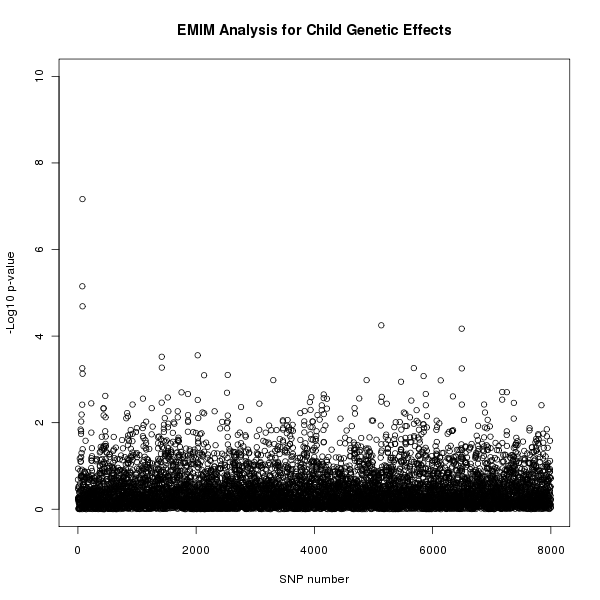
\includegraphics[width=200pt]{plotChildEffects.png}}
\caption{Plot of the -log10 p-values for each SNP given by EMIM to detect child genetic effects.}
\label{childeffs-fig}
\end{center}}
\end{figure}
}

If you wish to merge in the original SNP names as specified in the PLINK map file {\it exampleEMIM.bim}, and output a new summary file that includes a column with this information, as well as the p-values, you could do this in R using the following commands: 
\vspace{0.35cm} \begin{lstlisting}

snplist<-read.table("snplist.txt", header=F)
names(snplist)<-c("snpno","snpname","riskallele")
newsummary<-data.frame(snplist, pvaluesCG, resultsCG)
write.table(newsummary, file="emimnewsummaryCG.out", row.names=F, quote=F)

\end{lstlisting} \vspace{0.35cm}
Because of the way that PREMIM uses the SNP number as the SNP ID to be supplied to EMIM, you should find that the columns headed "snpno", "snp", "snpID" all correspond to the SNP number (order) in the original PLINK file {\it exampleEMIM.bim}, while the column headed "snpname" corresponds to its original name (e.g. an rsID) in the file {\it exampleEMIM.bim}. 

\subsubsection{Maternal Genetic Effects}
\label{eg-maternal}

Of course, we wish to use EMIM to test for effects other than child genetic effects. Now that PREMIM has already created the files that we need, to perform another analysis we can take the following steps to test for maternal genetic effects. 
\begin{enumerate}

\item {\bf Edit the EMIM parameter file.} To perform a maternal genetic effect analysis we firstly need to edit the {\it emimparams.dat} file, changing the following lines. \vspace{0.35cm} \begin{lstlisting}

...
0       << estimate R1 (0=no, 1=yes)
0       << estimate R2 (0=no, 1=yes)
...
1       << estimate S1 (0=no, 1=yes)
1       << estimate S2 (0=no, 1=yes)
...

\end{lstlisting} \vspace{0.35cm}Again, it may be useful to save a copy of the parameter file for future use. \vspace{0.35cm} \begin{lstlisting}

cp emimparams.dat emimparamsMG.dat

\end{lstlisting} \vspace{0.35cm}
\item {\bf Run EMIM.} Now that all the files are ready to perform a maternal genetic effects analysis we can run EMIM. \vspace{0.35cm} \begin{lstlisting}

./emim

\end{lstlisting} \vspace{0.35cm}
\item {\bf Analysis results.} As before, the results are output to files {\it emimresults.out} and {\it emimsummary.out}. We save these files for future use. \vspace{0.35cm} \begin{lstlisting}

cp emimsummary.out emimsummaryMG.out
cp emimresults.out emimresultsMG.out

\end{lstlisting} \vspace{0.35cm}We can view the results of the analysis in R using the following commands. \vspace{0.35cm} \begin{lstlisting}

# Read in the maternal analysis results:
resultsMG<-read.table("emimsummaryMG.out", header=T)

# Get the log likelihood ratio tests for each SNP
logLikeRatioMG<-resultsMG$twicediff

# Calculate the p-values for each SNP (2 degrees of freedom)
pvaluesMG<-1-pchisq(logLikeRatioMG, 2)

# Plot the -log10 p-values for each SNP
plot(resultsMG$snp, -log10(pvaluesMG), xlab="SNP number",
 ylab="-Log10 p-value",
 main="EMIM Analysis for Maternal Genetic Effects", ylim=c(0, 10) )

\end{lstlisting} \vspace{0.35cm}The results of this analysis can be seen in figure  \ref{mateffs-fig}. The plot appears to shows a maternal genetic effect later in the SNP sequence.\end{enumerate}
{\begin{figure}[ht]
{\begin{center}
{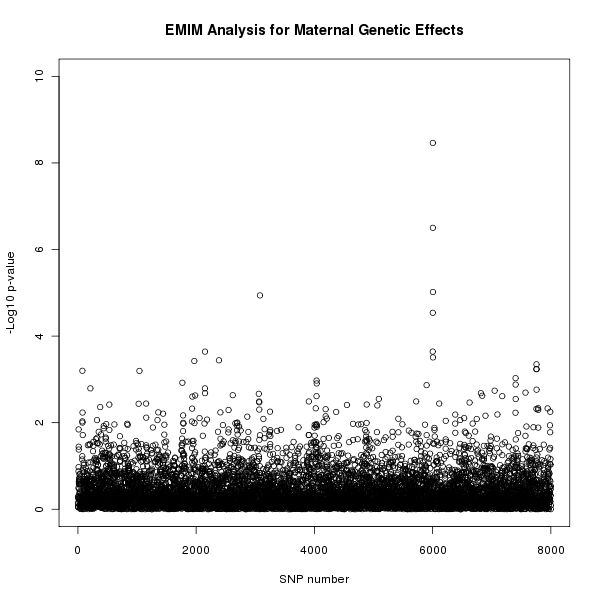
\includegraphics[width=200pt]{plotMaternalEffects.png}}
\caption{Plot of the -log10 p-values for each SNP given by EMIM to detect maternal genetic effects.}
\label{mateffs-fig}
\end{center}}
\end{figure}
}

%====== End of subsubsection "eg-maternal"======

\subsubsection{Maternal Genetic Effects Allowing for Child Genetic Effects}
\label{eg-maternal-wo-child}

We may wish to confirm that a maternal genetic effect is a genuine maternal genetic effect and not the result of an underlying child genetic effect. To test this we can take our null hypothesis to be the child genetic effect analysis and the alternative hypothesis to be the joint child and maternal genetic effect analysis. Firstly, we need to perform another EMIM analysis testing for both child and maternal genetic effects. 
\begin{enumerate}

\item {\bf Edit the EMIM parameter file.} To test for child and maternal genetic effects we firstly need to edit the {\it emimparams.dat} file, changing the following lines. \vspace{0.35cm} \begin{lstlisting}

...
1       << estimate R1 (0=no, 1=yes)
1       << estimate R2 (0=no, 1=yes)
...
1       << estimate S1 (0=no, 1=yes)
1       << estimate S2 (0=no, 1=yes)
...

\end{lstlisting} \vspace{0.35cm}Again, it may be useful to save a copy of the parameter file for future use. \vspace{0.35cm} \begin{lstlisting}

cp emimparams.dat emimparamsCGMG.dat

\end{lstlisting} \vspace{0.35cm}
\item {\bf Run EMIM.} Now that all the files are ready to perform a child and maternal genetic effects analysis we can run EMIM. \vspace{0.35cm} \begin{lstlisting}

./emim

\end{lstlisting} \vspace{0.35cm}
\item {\bf Analysis results.} Again, the results are output to files {\it emimresults.out} and {\it emimsummary.out}. We save these files for future use. \vspace{0.35cm} \begin{lstlisting}

cp emimsummary.out emimsummaryCGMG.out
cp emimresults.out emimresultsCGMG.out

\end{lstlisting} \vspace{0.35cm}We can view the results of the analysis for maternal effects whilst allowing for child effects by comparing the two EMIM analyses by using the following R commands: \vspace{0.35cm} \begin{lstlisting}

# Read in the results:
resultsCG<-read.table("emimsummaryCG.out", header=T)
resultsCGMG<-read.table("emimsummaryCGMG.out", header=T)

# Calculate the log likelihood ratio tests for each SNP
logLikeRatioCGMGvsCG<-2*(resultsCGMG$lnlikfull-resultsCG$lnlikfull)

# Calculate the p-values for each SNP (2 degrees of freedom)
pvaluesCGMGvsCG<-1-pchisq(logLikeRatioCGMGvsCG, 2)

# Plot the -log10 p-values for each SNP
plot(resultsCG$snp, -log10(pvaluesCGMGvsCG), xlab="SNP number",
 ylab="-Log10 p-value",
 main="EMIM Analysis for Maternal Genetic Effects allowing for Child Genetic Effects",
 ylim=c(0, 10) )

\end{lstlisting} \vspace{0.35cm}The results of this analysis can be seen in figure  \ref{matnotchildeffs-fig}. The plot appears to shows a maternal genetic effect later in the SNP sequence, further supporting the result shown in figure  \ref{mateffs-fig} that this effect is a genuine maternal genetic effect and not a child genetic effect.\end{enumerate}
{\begin{figure}[ht]
{\begin{center}
{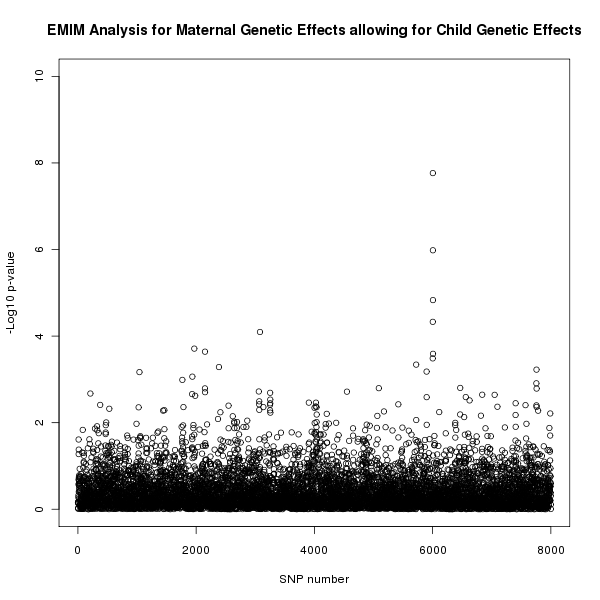
\includegraphics[width=200pt]{plotMaternalwoChildEffects.png}}
\caption{Plot of the -log10 p-values for each SNP given by EMIM to detect maternal genetic effects whilst allowing for child effects.}
\label{matnotchildeffs-fig}
\end{center}}
\end{figure}
}

%====== End of subsubsection "eg-maternal-wo-child"======

\subsubsection{Child Genetic Effects Allowing for Maternal Genetic Effects}
\label{eg-child-wo-maternal}

Similarly, we can test for child genetic effects whilst allowing for maternal genetic effects. We already have the results that we need from EMIM for this analysis, one for maternal genetic effects, which in this case we take as our null hypothesis, and another for child and maternal effects together, which is our alternative hypothesis. To view the results of this analysis we can use the following R commands. 
\vspace{0.35cm} \begin{lstlisting}

# Read in the results:
resultsMG<-read.table("emimsummaryMG.out", header=T)
resultsCGMG<-read.table("emimsummaryCGMG.out", header=T)

# Calculate the log likelihood ratio tests for each SNP
logLikeRatioCGMGvsMG<-2*(resultsCGMG$lnlikfull-resultsMG$lnlikfull)

# Calculate the P-values for each SNP (2 degrees of freedom)
pvaluesCGMGvsMG<-1-pchisq(logLikeRatioCGMGvsMG, 2)

# Plot the -log10 p-values for each SNP
plot(resultsMG$snp, -log10(pvaluesCGMGvsMG), xlab="SNP number",
 ylab="-Log10 p-value",
 main="EMIM Analysis for Child Genetic Effects allowing for Maternal Genetic Effects",
 ylim=c(0, 10) )

\end{lstlisting} \vspace{0.35cm}
The results of this analysis can be seen in figure  \ref{childnotmateffs-fig}. The plot appears to shows a child genetic effect early in the SNP sequence, this time supporting the result in figure  \ref{childeffs-fig} that this effect is a genuine child genetic effect and not a maternal genetic effect. 
{\begin{figure}[ht]
{\begin{center}
{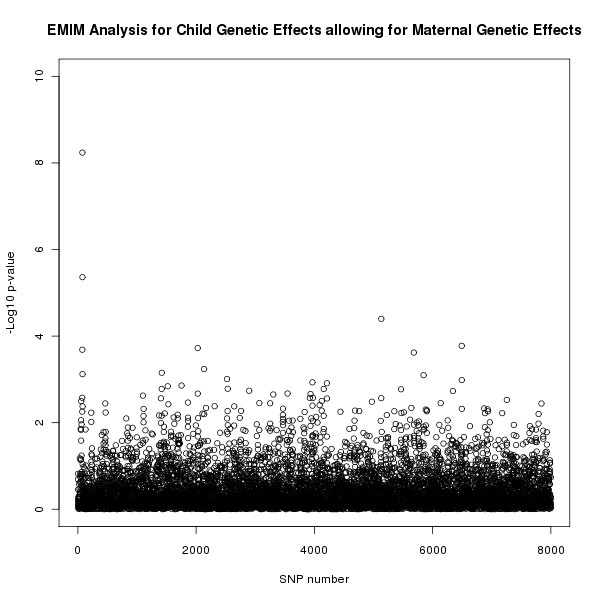
\includegraphics[width=200pt]{plotChildwoMaternalEffects.png}}
\caption{Plot of the -log10 p-values for each SNP given by EMIM to detect child genetic effects whilst allowing for maternal effects.}
\label{childnotmateffs-fig}
\end{center}}
\end{figure}
}

%====== End of subsubsection "eg-child-wo-maternal"======


In fact, these data were simulated to have a child genotype effect at SNP number 76 with $R_1 = 1.5$ and $R_2 = 2.25$ and a maternal genotype effect at SNP number 6004 with $S_1 = 2$ and $S_2 = 3$. 

%============ End of subsection "eg-run-emim"============


%================== End of section "example"==================

\section{Parallel processing}
\label{parallel}

EMIM performs the analysis for each SNP one by one, so if there are many SNPs then this may take a long time. It is therefore natural to want to speed up the process by performing these calculations in parallel. To facilitate this, EMIM and PREMIM have added features to make this easy by splitting the input files for EMIM into many different files, or by using multiple files (e.g. one file per chromosome) that have already been created using some other program such as PLINK. 

The following the instructions explain how to do this: 
\begin{enumerate}

\item {\bf Create input and output sub-directories for EMIM.} In the directory where your pedigree file or pedigree files are, create sub-directories for the input and output of EMIM. For example, to create directories simply called \code{input} and \code{output} in Linux/UNIX type: \vspace{0.35cm} \begin{lstlisting}

mkdir input
mkdir output

\end{lstlisting} \vspace{0.35cm}
\item {\bf Create input files for EMIM.} The next step is to create the input files for EMIM using PREMIM with your pedigree file(s). There are two different ways to do this: \begin{enumerate}

\item If your data is currently contained in a single file (e.g. called {\it data.bed}), you can use PREMIM with the "\code{-s n dir}" option to split the output files ({\it caseparenttrios.dat} etc.) into many files each containing \code{n} SNPs into directory \code{dir}. Since the data may be split into many files it is wise to put them in the separate \code{input} directory you made, in order to make them easier to manage. For example, to split the output into files each containing 1000 SNPs into the directory \code{input}, using the initial binary pedigree file {\it data.bed} and asking PREMIM to estimate allele frequencies, type: \vspace{0.35cm} \begin{lstlisting}
./premim -a -s 1000 input/ data.bed 
\end{lstlisting} \vspace{0.35cm}Note that the "/" is required after the directory name and a "\" may be required for systems other than Linux/UNIX. The files created will be named {\it input/caseparenttrios1.dat, input/caseparenttrios2.dat...} etc. Only one EMIM parameter file ({\it emimparams.dat}) is created (in the directory above the \code{input} directory). \\\\
\item If your data is already split into many files (e.g. one per chromosome, named {\it chr1.bed, chr2.bed, chr3.bed} etc.) you need to move these files into the \code{input} directory and, within the \code{input} directory, run PREMIM on each file to create the input files for EMIM. This can be done manually, one file at a time, or else you can write a loop via a Perl script or similar. Alternatively, if you are using a High Performance Computing (HPC) cluster using the open-source Sun Grid Engine (SGE) scheduler software, then these jobs may be submitted as an array job using something similar to the following script: \vspace{0.35cm} \begin{lstlisting}

#!/bin/bash
# execute in current working directory
#$ -cwd
# export local envirnoment
#$ -V
# the number of PREMIM tasks 
#$ -t 1-22
# execute PREMIM for each task
./premim -a -n $SGE_TASK_ID chr$SGE_TASK_ID.bed 

\end{lstlisting} \vspace{0.35cm}The key thing is to make sure that you use PREMIM's \code{-n} option to output a set of input files for EMIM which have different names (e.g. one set of EMIM input files per chromosome). This relies on the fact that it is possible to create files {\it caseparenttriosXXX.dat, caseparentsXXX.dat...} etc. in PREMIM by using the "\code{-n name}" option. For example to create output files with 5 appended to the end using pedigree file \code{data.ped}, you can type "\code{./premim -n 5 data.ped}" \\\\If the above job script is called {\it premimarray.sh} then it is submitted to the job queue as follows: \vspace{0.35cm} \begin{lstlisting}
qsub premimarray.sh 
\end{lstlisting} \vspace{0.35cm}This will submit a number of serial jobs (22 in the example above) to the HPC to execute in parallel. The exact details of how to perform parallel jobs may depend on your local computing services and you should consult your local computing support if in doubt. \\\\Once the array job, or Perl loop, or manual running of PREMIM has finished, you should have created a set of input files named {\it input/caseparenttrios1.dat, input/caseparenttrios2.dat...} etc. Only one EMIM parameter file ({\it emimparams.dat}) will have been created, corresponding to the last set of input files PREMIM created. This is not entirely satisfactory, as you may find that the last set of input files does not contain the largest number of SNPs. You therefore need to edit the number of SNPs on line 13 of {\it emimparams.dat} to the correspond to a number greater than the number of lines in the largest input file {\it emimmarkers*.dat}. E.g. type \vspace{0.35cm} \begin{lstlisting}

wc -l emimmarkers*.dat

\end{lstlisting} \vspace{0.35cm}to find out which file has the greatest number of lines, and edit the number of SNPs on line 13 of {\it emimparams.dat} to correspond to this number (or greater). THEN MOVE THIS FILE {\it emimparams.dat} ONE LEVEL BACK IN THE DIRECTORY HIERARCHY (i.e. it should be placed in the directory above the \code{input} directory).\end{enumerate}

\item {\bf Create SNP marker files.} Before running EMIM it must be ensured that the necessary SNP marker files are available for each set of input files. Normally the file {\it emimmarkers.dat} is used, in the parallel version the files {\it emimmarkers1.dat, emimmarkers2.dat...} etc. are used instead and are stored in the input directory for EMIM along with the rest of the files. If you used PREMIM's \code{-a} option when creating the input files for EMIM, then you should already have a usable set of SNP marker files in the \code{input} directory. Otherwise, these files may be created using an existing SNP marker file by using PREMIM with the "\code{-fm n markerfile.dat dir}" option which splits an existing marker file into many marker files each with \code{n} SNPs into directory \code{dir}. For example, to split the file {\it emimmarkers.dat} into marker files with 1000 SNPs each into directory \code{input} type: \vspace{0.35cm} \begin{lstlisting}
./premim -fm 1000 emimmarkers.dat input/ 
\end{lstlisting} \vspace{0.35cm}This creates the files {\it input/emimmarkers1.dat, input/emimmarkers2.dat...} etc. 
\item {\bf Run EMIM in parallel.} For each set of input files, for example, {\it input/caseparenttrios5.dat, input/caseparents5.dat...} etc., it is possible to run EMIM by typing: \vspace{0.35cm} \begin{lstlisting}
./emim 5 input/ output/ 
\end{lstlisting} \vspace{0.35cm}This will create result files {\it output/emimsummary5.out} and {\it output/emimresults5.out}. This must be done for every set of files numbered 1 to \code{N} for some \code{N}. The number \code{N} may correspond to 22 (e.g. if your data files were set up one per chromosome, for 22 chromosomes) or to some other number, depending on how many sets of input files were created by PREMIM when it split up your original data file. If you are using a High Performance Computing (HPC) cluster using the open-source Sun Grid Engine (SGE) scheduler software, then these jobs may be submitted as an array job using something similar to the following script: \vspace{0.35cm} \begin{lstlisting}

#!/bin/bash
# execute in current working directory
#$ -cwd
# export local envirnoment
#$ -V
# the number of EMIM tasks 
#$ -t 1-1435
# execute EMIM for each task
./emim $SGE_TASK_ID input/ output/

\end{lstlisting} \vspace{0.35cm}If the above script is saved in the directory above the \code{input} directory (i.e. the directory where your file {\it emimparams.dat} exists) and if the script is called {\it emimarray.sh}, then it is submitted to the job queue as follows: \vspace{0.35cm} \begin{lstlisting}
qsub emimarray.sh 
\end{lstlisting} \vspace{0.35cm}This will submit a number of serial jobs (1435 in the example above) to the HPC to execute in parallel. The exact details of how to perform parallel jobs may depend on your local computing services and you should consult your local computing support if in doubt. 
\item {\bf Collate EMIM results.} The results of the EMIM analysis are stored in the given output directory, for example {\it output/emimsummaryJ.out} and {\it output/emimresultsJ.out} for \code{J} from 1 to \code{N} for some \code{N}. This can be convenient if each file corresponds to a different chromosome, for example, but it is not very convenient if there are hundreds or thousands of result files. These files may therefore be collated into two result files {\it emimsummary.out} and {\it emimresults.out} by using the "\code{-fr dir}" option in PREMIM. For example, if the results are in directory \code{output} type: \vspace{0.35cm} \begin{lstlisting}
./premim -fr output/ 
\end{lstlisting} \vspace{0.35cm}Note that the SNP numbers in these combined files will relate to the number within each output file {\it output/emimsummaryJ.out} and {\it output/emimresultsJ.out}, which in turn corresponds to the SNP number within the input files {\it input/caseparenttriosJ.dat, input/casemotherduosJ.dat...} etc. As a result, these SNP numbers in the combined files will not be unique. If you used PREMIM to split a single file (e.g. {\it data.bed}) into many files for parallel processing, the SNP ID (as opposed to the SNP number) in the combined files should correspond to the SNP number within the original file {\it data.bed}, and so will be unique. If you used PREMIM to process a set of files (e.g. one per chromosome, named {\it chr1.bed, chr2.bed, chr3.bed} etc.) then both the SNP number and the SNP ID within the combined will not be unique, as they will refer to the number within the original file {\it chr1.bed, chr2.bed, chr3.bed} etc. We recommend you keep a separate list of the SNP identifiers from your .map or .bim files (e.g. their rs IDs) and their SNP number (order) within these files, in order to make it easier to match up the results in your combined output files with the correct SNPs. This can be done using the \code{-rout} option in PREMIM.\end{enumerate}

%================== End of section "parallel"==================

\section{Parent-of-origin effects with SHAPEIT2}
\label{poo}

{\bf Please download} the latest version of PREMIM if you have been running parent-of-origin analysis using SHAPEIT2 (version < 3.2) for important updates. These regard the combination of phased and non-phased data and do not affect data with only case/parent trios and case/duos. 

Parent-of-origin (or imprinting) effects relate to the situation where traits are influenced by the allele inherited from only one parent, with the allele from the other parent giving no effect. In most case/parent trio genotype combinations, the parent-of-origin can be deduced unambiguously, allowing investigation of such effects. However, when all three people are heterozygous, parent-of-origin cannot be determined. Existing methods operate on a SNP-by-SNP basis and either perform some sort of ``averaging'' or discard these ambiguous cases. If the correct parent-of-origin at a SNP could be determined then this would provide extra information and increase the power to detect imprinting effects. 

We have extended PREMIM/EMIM to make use of haplotype estimation in case/parent trios and duos, using surrounding SNP information for each SNP across the genome, as a means of estimating the parent-of-origin of alleles. PREMIM incorporates haplotype estimation performed by SHAPEIT2, see \citet{delaneau:etal:12} and \citet{delaneau:etal:13}. SHAPEIT2 can be downloaded from the SHAPEIT website (www.shapeit.fr). 

You can use PREMIM and EMIM with SHAPEIT2 by running \code{PREMIM} with the \code{-ihap} option and using the \code{-shapeit} option to indicate the command (with full pathname if required) on your system to run SHAPEIT2. 
\vspace{0.35cm} \begin{lstlisting}
./premim -a -ihap -shapeit ./shapeit2 mydata.bed

./emim

\end{lstlisting} \vspace{0.35cm}
See \citet{howey:etal:15} for a more in-depth account of the methodology. 
\subsection{Options}
\label{options}

The additional options for using PREMIM with SHAPEIT2 to estimate the parent-of-origin of alleles are summarised below: 

{\begin{center}\begin{tabular}{ll}
Option  & Description\\
\hline
-ihap  & estimate haplotypes for improved modelling of imprinting (not permitted with the -xa option)\\
-ihap-noadj  & do not adjust estimated duo cell counts\\
-ihap-miss-thres h  & maximum missing data threshold, h, for trios and duos (default h=0.5)\\
-shapeit com  & shapeit command with full path if required (default com=``shapeit2'')\\
-shapeit-thread t  & shapeit thread option: --thread t (default t=12)\\
-shapeit-mcmc-ops b p m  & shapeit MCMC options: --burn b --prune p --main m (default b=7, p=8, m=20)\\
-shapeit-model-ops s w  & shapeit model options: --states s --window w (defualt s=100, w=2)\\
-shapeit-ops ``options''  & other shapeit options, use ``'' to surround options\\
\end{tabular}\end{center}}

Various options can be set when SHAPEIT2 estimates the haplotypes via PREMIM, it is recommended to keep the default settings unless you have specific reason to change them for your particular analysis. If more than 12 processors are available then it would beneficial to increase the number of threads to speed up haplotype estimation. The \code{-shapeit-ops} option allows any parameters to be set with SHAPEIT2 to estimate the haplotypes, for example to use a reference panel and 15 threads: 
\vspace{0.35cm} \begin{lstlisting}
./premim -a -ihap -shapeit ./shapeit2 -shapeit-thread 15 -shapeit-ops "--input-ref ref.haplotypes.gz ref.legend.gz ref.sample" mydata.bed

./emim

\end{lstlisting} \vspace{0.35cm}
%============ End of subsection "options"============

\subsection{Data files}
\label{files}

The input data files for using EMIM with estimated parent-of-origin alleles for case/parent trios, case/mother duos and case/father duos are different from the usual EMIM input files. The case/parent trios have 4 extra columns and look something like the following: 
\vspace{0.35cm} \begin{lstlisting}
snp	cellcount 1-15 (+2 phased, +2 totals)
1	21 38 41 34 38 78 73 73 0 68 147 146 149 147 281 88 78 0 1500
2	51 85 75 71 76 88 84 91 0 94 120 115 105 102 138 89 116 0 1500
3	18 39 38 44 39 69 68 79 0 81 148 161 134 156 253 88 85 0 1500
4	1 16 14 20 14 48 47 59 0 66 160 182 151 163 448 55 56 0 1500
5	1 7 7 9 6 38 33 41 0 47 151 170 147 163 597 43 40 0 1500
6	1 4 3 3 3 26 24 31 0 35 141 156 137 150 726 29 31 0 1500
7	0 1 3 2 1 14 17 15 0 22 119 131 115 126 898 15 21 0 1500
8	0 1 1 1 1 3 10 4 0 8 98 110 91 99 1058 8 7 0 1500
...

\end{lstlisting} \vspace{0.35cm}
The first 16 columns are the same as before, see  section \ref{caseparenttrios} for details. The last 4 columns are: 
\begin{enumerate}

\item 9a cell count - the estimated number of genotypes with the risk allele inherited from the {\bf father} in the ambiguous scenario of all heterogenous individuals. 
\item 9b cell count - the estimated number of genotypes with the risk allele inherited from the {\bf mother} in the ambiguous scenario of all heterogenous individuals. 
\item The total number of case/parent trios not phased. 
\item The total number of case/parent trios phased.\end{enumerate}

{\bf Note} that since, when using PREMIM and SHAPEIT2 to create these files, all case/parent trios are phased, cell 9 is always 0. In principle, for analysis in EMIM, one can combine data sets where phasing has/has not been performed. In that situation, cell 9 would not necessarily be equal to 0. 

The case/mother duos also have 4 extra columns and will look something like the following: 
\vspace{0.35cm} \begin{lstlisting}

snp	cellcount 1-7 (+2 phased, +2 totals)
1	43 133 127 0 219 225 428 100.1 224.9 0 1500
2	128 188 201 0 209 206 246 158.805 163.195 0 1500
3	62 134 137 0 222 231 400 112.655 201.345 0 1500
4	15 76 84 0 191 212 647 70.8306 204.169 0 1500
5	7 46 58 0 174 204 771 40.6535 199.346 0 1500
6	5 30 37 0 154 175 904 28.2062 166.794 0 1500
7	3 24 16 0 120 148 1032 17.1744 139.826 0 1500
8	2 11 7 0 83 105 1181 8.23184 102.768 0 1500
9	57 128 125 0 189 209 461 120.105 210.895 0 1500
...

\end{lstlisting} \vspace{0.35cm}
Similarly, the case/father duos also have 4 extra columns and will look something like the following: 
\vspace{0.35cm} \begin{lstlisting}

snp	cellcount 1-7 (+2 phased, +2 totals)
1	55 113 128 0 213 230 420 226.766 114.234 0 1500
2	131 166 157 0 216 227 253 191.468 158.532 0 1500
3	67 116 119 0 214 226 439 211.791 107.209 0 1500
4	19 69 76 0 198 196 653 215.963 73.0372 0 1500
5	7 47 61 0 172 182 774 202.364 54.6364 0 1500
6	4 31 39 0 155 170 887 178.309 35.6908 0 1500
7	1 15 26 0 119 139 1025 158.154 16.8459 0 1500
8	0 7 11 0 92 97 1174 110.437 8.56334 0 1500
9	60 120 101 0 198 252 415 238.776 115.224 0 1500
...

\end{lstlisting} \vspace{0.35cm}
The first 8 columns for case/mother duos and case/father duos are the same as before, see  section \ref{casemotherduos} and  section \ref{casefatherduos} respectively for details. The last 4 columns are: 
\begin{enumerate}

\item 4a cell count - the estimated number of genotypes with the risk allele inherited from the {\bf father} in the ambiguous scenario of both heterogenous individuals. 
\item 4b cell count - the estimated number of genotypes with the risk allele inherited from the {\bf mother} in the ambiguous scenario of both heterogenous individuals. 
\item The total number of duos not phased. 
\item The total number of duos phased.\end{enumerate}

Note that the estimates for the duos are not integers as the estimated cell counts are adjusted by PREMIM to avoid potential type I error problems, see \citet{howey:etal:15} for more details. 

It is necessary to tell EMIM that it will be analysing this extended data and the start of the EMIM parameter file, \code{emimparams.dat}, should be something as follows: 
\vspace{0.35cm} \begin{lstlisting}
-----------INPUT DATAFILES------------------------------------------------
2   << caseparenttrios.dat file (0=no, 1=yes, 2=yes, using haplotype estimates)
0   << caseparents.dat file (0=no, 1=yes)
2   << casemotherduos.dat file (0=no, 1=yes, 2=yes, using haplotype estimates)
2   << casefatherduos.dat file (0=no, 1=yes, 2=yes, using haplotype estimates)
0   << casemothers.dat file (0=no, 1=yes)
...

\end{lstlisting} \vspace{0.35cm}
The parameter file is automatically produced as such by PREMIM if SHAPEIT2 is used. 
\subsubsection{Combining Data}
\label{combining-data}

It is possible to combine two EMIM data files simply by adding the cell counts together. This could be done for one data set that has been phased and another that has not been phased. If this is done then it is also necessary to update the 2 total columns. Obviously, the list of SNPs in each of the two files must match. 

The following R code demonstrates how some unphased data in the old EMIM format could be combined with some phased data in the new EMIM format: 
\vspace{0.35cm} \begin{lstlisting}
## Read in unphased case/parent trios and skip header
caseparenttrios.unphased<-read.table("unphased-data/caseparenttrios.dat", skip=1)

## Convert data to the new EMIM format
cell9a<-rep(0, length(caseparenttrios.unphased[,1]))
cell9b<-rep(0, length(caseparenttrios.unphased[,1]))
total.unphased<-rowSums(caseparenttrios.unphased[,2:16])
total.phased<-rep(0, length(caseparenttrios.unphased[,1]))

## Put unphased data into the new format
caseparenttrios.newformat<-cbind(caseparenttrios.unphased, cell9a, cell9b, total.unphased, total.phased) 

## Read in phased case/parent trios and skip header
caseparenttrios.phased<-read.table("phased-data/caseparenttrios.dat", skip=1)

## Check data is the same size
dim(caseparenttrios.phased)
dim(caseparenttrios.newformat)

## Combine the data
combined.data<-caseparenttrios.newformat + caseparenttrios.phased

## Set snp number correctly
combined.data[,1]<-1:length(combined.data[,1])

## Write new combined data, the header is not important except there must be one
write.table(combined.data, "combined-data/caseparenttrios.dat", row.names=FALSE, col.names=TRUE, quote=FALSE)

\end{lstlisting} \vspace{0.35cm}
For example, the unphased case/parent trios data may look as follows: 
\vspace{0.35cm} \begin{lstlisting}
snp	cellcount 1-15
1      4 10 17 9 13 6 4 14 44 26 25 17 24 12 19
2      1 0 8 0 5 2 3 2 23 21 29 38 26 43 52
3      0 0 0 0 0 0 0 0 0 1 1 0 1 0 319
4      0 0 3 0 0 2 4 1 13 24 22 40 8 25 131
5      0 0 5 3 6 4 7 2 23 23 29 44 19 46 59
6      0 0 1 2 0 0 2 2 4 8 14 18 21 26 197
7      0 0 3 0 0 1 0 1 11 18 14 37 12 29 160
8      1 3 9 5 12 9 8 12 31 30 28 26 31 20 20
...

\end{lstlisting} \vspace{0.35cm}
and the phased case/parent trios data as follows: 
\vspace{0.35cm} \begin{lstlisting}
snp	cellcount 1-15 (+2 phased, +2 totals)
1	9 20 27 20 18 37 36 35 0 30 70 64 65 75 121 38 35 0 700
2	28 40 29 33 36 39 44 39 0 45 49 47 60 36 62 58 55 0 700
3	14 17 14 17 18 38 41 40 0 47 65 62 69 54 116 49 39 0 700
4	6 5 7 4 9 24 28 25 0 24 63 82 82 78 210 32 21 0 700
5	3 5 2 4 5 21 21 14 0 19 57 82 79 70 282 19 17 0 700
6	2 0 1 2 2 15 20 10 0 14 56 68 70 63 351 16 10 0 700
7	1 1 0 0 2 10 9 4 0 10 47 57 60 55 428 6 10 0 700
8	0 2 0 0 1 2 5 1 0 8 33 44 43 39 511 4 7 0 700
...

\end{lstlisting} \vspace{0.35cm}
resulting in combined case/parent trios data: 
\vspace{0.35cm} \begin{lstlisting}
V1 V2 V3 V4 V5 V6 V7 V8 V9 V10 V11 V12 V13 V14 V15 V16 cell9a cell9b total.unphased total.phased
1 13 30 44 29 31 43 40 49 44 56 95 81 89 87 140 38 35 244 700
2 29 40 37 33 41 41 47 41 23 66 78 85 86 79 114 58 55 253 700
3 14 17 14 17 18 38 41 40 0 48 66 62 70 54 435 49 39 322 700
4 6 5 10 4 9 26 32 26 13 48 85 122 90 103 341 32 21 273 700
5 3 5 7 7 11 25 28 16 23 42 86 126 98 116 341 19 17 270 700
6 2 0 2 4 2 15 22 12 4 22 70 86 91 89 548 16 10 295 700
7 1 1 3 0 2 11 9 5 11 28 61 94 72 84 588 6 10 286 700
8 1 5 9 5 13 11 13 13 31 38 61 70 74 59 531 4 7 245 700
...

\end{lstlisting} \vspace{0.35cm}
Do not worry about the weird header, this can be anything, but there must be a header as EMIM expects one (which it will ignore!). 

Similarly, the case/mother duos can be combined using the following R code: 
\vspace{0.35cm} \begin{lstlisting}
## Read in unphased case/mother duos and skip header
casemotherduos.unphased<-read.table("unphased-data/casemotherduos.dat", skip=1)

## Convert data to the new EMIM format
cell4a<-rep(0, length(casemotherduos.unphased[,1]))
cell4b<-rep(0, length(casemotherduos.unphased[,1]))
total.unphased<-rowSums(casemotherduos.unphased[,2:8])
total.phased<-rep(0, length(casemotherduos.unphased[,1]))

## Put unphased data into the new format
casemotherduos.newformat<-cbind(casemotherduos.unphased, cell4a, cell4b, total.unphased, total.phased) 

## Read in phased case/mother duos and skip header
casemotherduos.phased<-read.table("phased-data/casemotherduos.dat", skip=1)
casemotherduos.phased<-casemotherduos.phased[1:8,]

## Check data is the same size
dim(casemotherduos.phased)
dim(casemotherduos.newformat)

## Combine the data
combined.data<-casemotherduos.newformat + casemotherduos.phased

## Set snp number correctly
combined.data[,1]<-1:length(combined.data[,1])

## Write new combined data, the header is not important except there must be one
write.table(combined.data, "combined-data/casemotherduos.dat", row.names=FALSE, col.names=TRUE, quote=FALSE)

\end{lstlisting} \vspace{0.35cm}
Similarly, for the case/father duos data. All other data files are all formatted in the old EMIM format and can be combined without any conversion. 

%====== End of subsubsection "combining-data"======


%============ End of subsection "files"============

\subsection{Example Analysis}
\label{poo-example}

This section demonstrates the use of PREMIM/EMIM with SHAPEIT2 to estimate the parent-of-origin of alleles through the use of an example. Data for this analysis uses simulated data with 700 case/parent trios, 500 case/maother duos, 250 case/father duos and 50 cases with 1000 SNPs. A causal SNP was set at SNP number 250 and the SNPs had a 3 percent missing data rate. The data can be downloaded here. 

Firstly ensure that you have a working version of SHAPEIT2 installed, currently only available for LINUX, and can be downloaded from here. 

The following PREMIM command uses the \code{-ihap} option to estimate the parent-of-origin of alleles with the local SHAPEIT2 command set with the \code{-shapeit} option, and \code{-a} to estimate risk allele frequencies and \code{-im} to set the EMIM parameter file to analysis maternal imprinting effects. 
\vspace{0.35cm} \begin{lstlisting}
./premim -a -im -ihap -shapeit /home/me/myprogs/shapeit2 demo-poo-data.bed 
\end{lstlisting} \vspace{0.35cm}
The output should appear something like the following: 
\vspace{0.35cm} \begin{lstlisting}
PREMIM: Pedigree file processing program for EMIM, v3.12
--------------------------------------------------------
Copyright 2011-2015 Richard Howey, GNU General Public License, v3
Institute of Genetic Medicine, Newcastle University

Log file: premim.log
Input file: demo-poo-data.bed
Maternal imprinting analysis set for parameter file (emimparams.dat).
Estimating allele frequencies and writing to file (emimmarkers.dat).
Estimating parent-of-origin with SHAPEIT2.
SHAPEIT2 command: /home/me/myprogs/shapeit2
Maximum missing data permitted for trios and duos: 0.5

Calculating haplotype graph using SHAPEIT command:
/home/me/myprogs/shapeit2 --input-bed tempForSHAPEIT.bed tempForSHAPEIT.bim tempForSHAPEIT.fam --output-graph tempOutSHAPEIT.hgraph 
  --output-log tempOutSHAPEIT-hgraph.log --thread 12 --burn 7 --prune 8 --main 20 --states 100 --window 2 >/dev/null 2>&1

Calculating haplotype estimates using SHAPEIT command:
/home/me/myprogs/shapeit2 -convert --input-graph tempOutSHAPEIT.hgraph --output-max tempOutSHAPEIT.haps tempOutSHAPEIT.sample 
  --output-log tempOutSHAPEIT-max.log  --thread 12 >/dev/null 2>&1

Case/mother duo adjustment parameters:
beta0 = 0.00753525
beta1 = -0.129427
beta2 = 0.560096
beta3 = -0.755696

Case/father duo adjustment parameters:
beta0 = -0.010869
beta1 = 0.183147
beta2 = -0.772304
beta3 = 0.986696


Number of subjects: 3650
          Males: 2450 (67.1233%)
          Females: 1200 (32.8767%)
          Unknown sex: 0 (0%)
          Affected: 1500 (41.0959%)
          Unaffected: 2150 (58.9041%)
Number of SNPs: 1000

Number of pedigrees: 1500
Mean pedigree size: 2.43333
Standard deviation of pedigree size: 0.558955

File name: emimmarkers.dat
Number of allele SNP frequencies estimated: 1000

File name: caseparenttrios
Number of counted case parent trios (all SNPs): 700000
Average number of counted case parent trios (per SNP): 700
Number of uncounted (Mendelian error) case parent trios: 0

File name: casemotherduos
Number of counted case mother duos (all SNPs): 500000
Average number of counted case mother duos (per SNP): 500
Number of uncounted (Mendelian error) case mother duos: 0

File name: casefatherduos
Number of counted case father duos (all SNPs): 250000
Average number of counted case father duos (per SNP): 250
Number of uncounted (Mendelian error) case father duos: 0

File name: cases
Number of counted cases (all SNPs): 48465
Average number of counted cases (per SNP): 48.465

File name: caseparents
Number of counted case parents (all SNPs): 0
Average number of counted case parents (per SNP): 0
Number of uncounted (Mendelian error) case parents: 0

File name: casemothers
Number of counted case mothers (all SNPs): 0
Average number of counted case mothers (per SNP): 0

File name: casefathers
Number of counted case fathers (all SNPs): 0
Average number of counted case fathers (per SNP): 0

File name: conparents
Number of counted control parents (all SNPs): 0
Average number of counted control parents (per SNP): 0
Number of uncounted (Mendelian error) control parents: 0

File name: conmotherduos
Number of counted control mother duos (all SNPs): 0
Average number of counted control mother duos (per SNP): 0
Number of uncounted (Mendelian error) control mother duos: 0

File name: confatherduos
Number of counted control father duos (all SNPs): 0
Average number of counted control father duos (per SNP): 0
Number of uncounted (Mendelian error) control father duos: 0

File name: cons
Number of counted controls (all SNPs): 0
Average number of counted controls (per SNP): 0

Number of uncounted groups: 1535

Run time: 6 minutes and 11 seconds

\end{lstlisting} \vspace{0.35cm}
This output should also be recorded in the \code{premim.log} file. 

Importantly, in the example above, the default \code{--thread 12} option for SHAPEIT2 was used to speed up the computation by running the analysis in parallel. This analysis took about 9 minutes on my computer, without the thread option you could expect it to take over 90 minutes! If more processes are available you can set this using the PREMIM option \code{-shapeit-thread 15} say. 

The >/dev/null 2>\&1bit shown in the output is to stop the screen output of SHAPEIT2. 

There are a number of files, \code{tempOutSHAPEIT*}, that are created and used during the estimation process and should have been automatically removed. For this reason you should not set off more than one job running at a time in the same directory 

The case/mother duos and case/father duos are adjusted separately and the regression parameters are expected to be zero if no adjustment were necessary. In this case the parameters are not near zero, indicating that an adjustment was necessary. Performing an adjustment is default since this does not reduce power but does reduce type I error. 

There are no missing case/parent trios or duos in the PREMIM summary data since SHAPEIT2 can impute missing data and a normal background missing data rate is not a problem. There are, however, some missing cases as with older versions of PREMIM. 

The next step is to check that the EMIM parameter file is set for the desired analysis. The parameter file \code{emimparams.dat} should appear as follows: 
\vspace{0.35cm} \begin{lstlisting}

-----------INPUT DATAFILES------------------------------------------------
2   << caseparenttrios.dat file (0=no, 1=yes, 2=yes, using haplotype estimates)
0   << caseparents.dat file (0=no, 1=yes)
2   << casemotherduos.dat file (0=no, 1=yes, 2=yes, using haplotype estimates)
2   << casefatherduos.dat file (0=no, 1=yes, 2=yes, using haplotype estimates)
0   << casemothers.dat file (0=no, 1=yes)
0   << casefathers.dat file (0=no, 1=yes)
1   << cases.dat file (0=no, 1=yes)
0   << conparents.dat file (0=no, 1=yes)
0   << conmotherduos.dat file (0=no, 1=yes)
0   << confatherduos.dat file (0=no, 1=yes)
0   << cons.dat file (0=no, 1=yes)
1000   << no of SNPs in each file
------------------PARAMETER RESTRICTIONS----------------------------------
0   << fix allele freq A (0=no, 1=yes)
1   << assume HWE and random mating (0=no=estimate 6 mu parameters, 1=yes)
0   << assume parental allelic exchangeability (0=no, 1=yes)
0   << use CPG likelihood (9 mu parameters)
0   << estimate R1 (0=no, 1=yes)
0   << estimate R2 (0=no, 1=yes)
0   << R2=R1 (0=no, 1=yes)
0   << R2=R1squared	(0=no, 1=yes)
0   << estimate S1 (0=no, 1=yes)
0   << estimate S2 (0=no, 1=yes)
0   << S2=S1 (0=no, 1=yes)
0   << S2=S1squared	(0=no, 1=yes)
1   << estimate Im (0=no, 1=yes)
0   << estimate Ip (0=no, 1=yes)
0   << estimate gamma11 (0=no, 1=yes)
0   << estimate gamma12 (0=no, 1=yes)
0   << estimate gamma21 (0=no, 1=yes)
0   << estimate gamma22 (0=no, 1=yes)
0   << gamma22=gamma12=gamma21=gamma11 (0=no, 1=yes)
---------------OTHER PARAMETERIZATIONS------------------------------------
0   << estimate Weinberg (1999b) Im (0=no, 1=yes)
0   << estimate Weinberg (1999b) Ip (=Li 2009 Jm) (0=no, 1=yes)
0   << estimate Sinsheimer (2003) gamma01 (0=no, 1=yes)
0   << estimate Sinsheimer (2003) gamma21 (0=no, 1=yes)
0   << estimate Palmer (2006) match parameter (0=no, 1=yes)
0   << estimate Li (2009) conflict parameter Jc (0=no, 1=yes)

\end{lstlisting} \vspace{0.35cm}
Note that the trio and duo data files are set to 2 to indicate that the extended data files with estimated parent-of-origin alleles must be used. If this is not set correctly to match the format of the data, the EMIM analysis will fail. We can take a copy of the parameter file for later use. 
\vspace{0.35cm} \begin{lstlisting}
cp emimparams.dat emimparamsIm.dat 
\end{lstlisting} \vspace{0.35cm}
Next, run the EMIM analysis: 
\vspace{0.35cm} \begin{lstlisting}
./emim 
\end{lstlisting} \vspace{0.35cm}
Save the results from this analysis for use later: 
\vspace{0.35cm} \begin{lstlisting}
mv emimsummary.out emimsummaryIm.out
mv emimresults.out emimresultsIm.out

\end{lstlisting} \vspace{0.35cm}
Start up R and then (within R) the results can then be inspected: 
\vspace{0.35cm} \begin{lstlisting}
## Read in the maternal imprinting effects analysis results:
resultsIm<-read.table("emimsummaryIm.out", header=TRUE)

## Get the log likelihood ratio tests for each SNP
logLikeRatioIm<-resultsIm$twicediff

## Calculate the p-values for each SNP (1 degree of freedom)
pvaluesIm<-pchisq(logLikeRatioIm, 1, lower.tail=FALSE)

## Do 2 plots
par(mfrow=c(1,2))

## Plot the -log10 p-values for each SNP
plot(resultsIm$snp, -log10(pvaluesIm), xlab="SNP number", ylab="-Log10 p-value", main="EMIM Analysis for Maternal Imprinting Effects")

## Remove any NA results (although none here)
chisqsIm<-logLikeRatioIm[!is.na(logLikeRatioIm)]

## Plot a Q-Q plot of the chi square test statistics
plot(qchisq(ppoints(chisqsIm), df=1), sort(chisqsIm), xlab="theoretical", ylab="observed", main="Q-Q Plot for Maternal Imprinting Effects")
abline(a=0, b=1, col="red")
     
## Calculate the inflation factor for 1 degree of freedom
median(chisqsIm)/0.456

## Find the SNP with the lowest p-value
min(pvaluesIm)

\end{lstlisting} \vspace{0.35cm}
The plots from the above analysis are shown in figure  \ref{poo-im-fig} and show the maternal imprinting effect around the causal SNP, with a p-value of 3.16e-13. The Q-Q plot is satisfactory with an inflation factor of 0.929. If you perform the same analysis with this data you should expect different, but similar, results. The inflation factor may be quite different but should be fairly close to 1 and the Q-Q plot should appear similar. SHAPEIT2 uses a stochastic Markov chain Monte Carlo (MCMC) process to phase the haplotypes and so the estimates will be slightly different each time, resulting in slightly different results in EMIM. In fact, since this a small simulated data set the phasing is not too accurate and so the results vary much more than with a large real data set. 
{\begin{figure}[ht]
{\begin{center}
{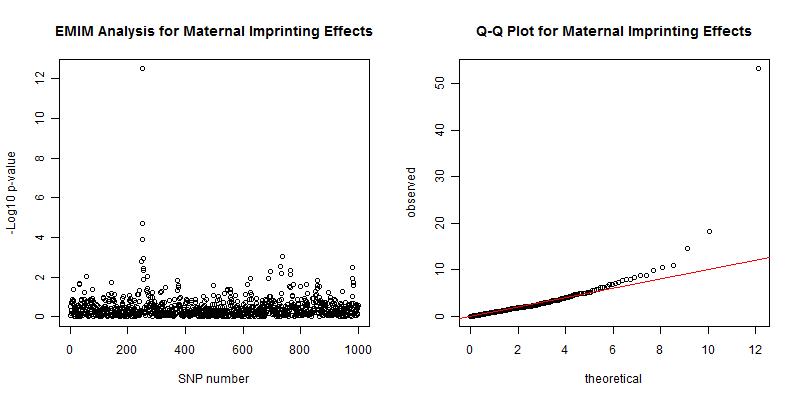
\includegraphics[width=400pt]{pooExampleDataIm.png}}
\caption{Left plot of the -log10 p-values for each SNP given by EMIM to detect maternal imprinting effects using alleles with SHAPEIT2 estimated parent-of-origins. Right plot show a Q-Q plot of the chi-square test statistics with an inflation factor of 0.929.}
\label{poo-im-fig}
\end{center}}
\end{figure}
}
\subsubsection{Maternal Imprinting Effects allowing for Child Genetic Effects}
\label{eg-maternal-imp-wo-child}

Next, we will perform an analysis to detect maternal effects while allowing for child genotype effects. Firstly, we create the two EMIM parameter files necessary to perform two EMIM analyses, one testing for maternal imprinting and child genotype effects and the other testing for only child genotype effects: 
\vspace{0.35cm} \begin{lstlisting}

cp emimparams.dat emimparamsImCG.dat  
cp emimparams.dat emimparamsCG.dat 

\end{lstlisting} \vspace{0.35cm}
The files should be edited so that \code{emimparamsImCG.dat} is such that: 
\vspace{0.35cm} \begin{lstlisting}

...
1   << estimate R1 (0=no, 1=yes)
1   << estimate R2 (0=no, 1=yes)
...
1   << estimate Im (0=no, 1=yes)
...

\end{lstlisting} \vspace{0.35cm}
and \code{emimparamsCG.dat} is as follows: 
\vspace{0.35cm} \begin{lstlisting}
... 
1   << estimate R1 (0=no, 1=yes)
1   << estimate R2 (0=no, 1=yes)
...
0   << estimate Im (0=no, 1=yes)
...

\end{lstlisting} \vspace{0.35cm}
Next, update the EMIM parameter file and test for maternal imprinting and child genotype effects: 
\vspace{0.35cm} \begin{lstlisting}
cp emimparamsImCG.dat emimparams.dat
./emim

\end{lstlisting} \vspace{0.35cm}
Save the results for later: 
\vspace{0.35cm} \begin{lstlisting}
mv emimsummary.out emimsummaryImCG.out
mv emimresults.out emimresultsImCG.out

\end{lstlisting} \vspace{0.35cm}
Now, test for child genotype effects in the same manner: 
\vspace{0.35cm} \begin{lstlisting}
cp emimparamsCG.dat emimparams.dat
./emim

mv emimsummary.out emimsummaryCG.out
mv emimresults.out emimresultsCG.out

\end{lstlisting} \vspace{0.35cm}
Start up R and then (within R) the results can then be inspected: 
\vspace{0.35cm} \begin{lstlisting}

## Read in the maternal imprinting effects and child genotype effects analysis results:
resultsImCG<-read.table("emimsummaryImCG.out", header=TRUE)
resultsCG<-read.table("emimsummaryCG.out", header=TRUE)

## Calculate the log likelihood ratio tests for each SNP
logLikeRatioImCGvsCG<-2*(resultsImCG$lnlikfull-resultsCG$lnlikfull)

## Calculate the p-values for each SNP (1 degree of freedom)
pvaluesImCGvsCG<-pchisq(logLikeRatioImCGvsCG, 1, lower.tail=FALSE)

## Do 2 plots
par(mfrow=c(1,2))

## Plot the -log10 p-values for each SNP
plot(resultsCG$snp, -log10(pvaluesImCGvsCG), xlab="SNP number", ylab="-Log10 p-value",
  main="Maternal Imprinting Effects\n allowing for Child Genetic Effects")

## Remove any NA results (although none here)
chisqsImCGvsCG<-logLikeRatioImCGvsCG[!is.na(logLikeRatioImCGvsCG)]

## Plot Q-Q plot of chi square test statistics
plot(qchisq(ppoints(chisqsImCGvsCG), df=1), sort(chisqsImCGvsCG), xlab="theoretical", ylab="observed",
  main="Q-Q Plot for Maternal Imprinting Effects\n allowing for Child Genetic Effects") 
abline(a=0,b=1, col="red")

## Calculate the inflation factor for 1 degree of freedom
median(chisqsImCGvsCG)/0.456

## Find the SNP with the lowest p-value
min(pvaluesImCGvsCG)

\end{lstlisting} \vspace{0.35cm}
The plots from the maternal imprinting while allowing for child genetic effects analysis are shown in figure  \ref{poo-imr-fig} and show that the maternal imprinting effect is still present around the causal SNP, with a p-value of 8.89e-8, and the Q-Q plot is also satisfactory with an inflation factor of 1.01. As before, if you perform this analysis the results will probably be different, due to the stochastic nature of the SHAPEIT2 algorithm. 
{\begin{figure}[ht]
{\begin{center}
{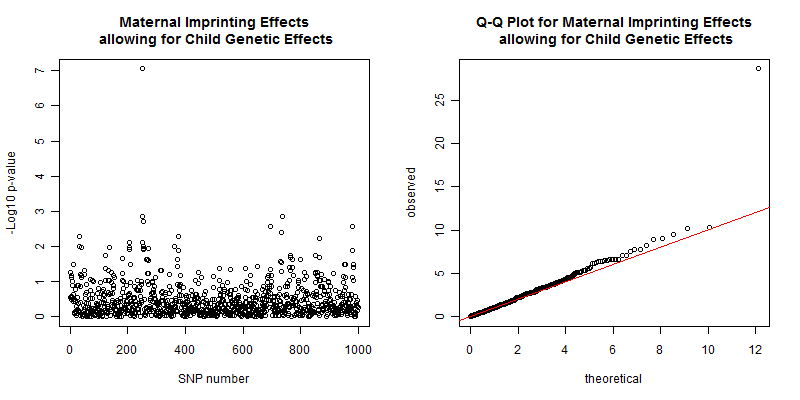
\includegraphics[width=400pt]{pooExampleDataImR.png}}
\caption{Left plot of the -log10 p-values for each SNP given by EMIM to detect maternal imprinting effects allowing for child genotype effects using alleles with SHAPEIT2 estimated parent-of-origins. Right plot show a Q-Q plot of the chi-square test statistics with an inflation factor of 1.01.}
\label{poo-imr-fig}
\end{center}}
\end{figure}
}

%====== End of subsubsection "eg-maternal-imp-wo-child"======


%============ End of subsection "poo-example"============


%================== End of section "poo"==================

\section{Troubleshooting and results interpretation}
\label{trouble}

PREMIM and EMIM are ideally designed for use by users who already have experience of analysing genetic data and some familiarity with using command-line programs such as PLINK, SNPTEST, MACH or IMPUTE. If you do not have any such experience, we recommend you attept to gain some familiarity with such programs before embarking on an analysis with PREMIM and EMIM. 

As with any other statistical analysis method, the results from EMIM are only as reliable as the quality of the data going in to the analysis. If you obtain "strange" results or get a warning/error message, by far the most likely reason is that there is some "problem" with the input data. By "problem", this could mean an actual mistake in the input files (e.g. they are not formatted correctly), or it could simply mean that there is limited information provided by the input data, or that the data is too noisy, to produce reliable/interpretable results. 

One common problem is that there is too little data to estimate the parameters requested. This could result from too many cells with zero observations in the input data files {\it caseparenttrios.dat}, {\it casemotherduos.dat} etc. We have tried to get EMIM to pick up these sorts of issues automatically and give a sensible warning message, but, given the complexities of the potential possible models, it does not always manage to achieve this! You may find that using a more restricted model (e.g. assuming HWE and random mating) helps with parameter identifiability/estimation problems. 

If you obtain "significant results" (that you either disbelieve - because they seem "too good to be true" - or believe, in the hope that they are true!) at one or more SNPs analysed, our first recommendation is to make a smaller input data set (e.g. using the \code{--extract snplist.txt} command in PLINK) consisting just of this subset of SNPs of interest, and re-run PREMIM and EMIM just on this subset of SNPs. This will allow you to examine the output file {\it emimresults.out} more carefully (normally this file is too big to easily sort through in order to find the results pertaining to one specific SNP). You should also carefully examine the last column of the file {\it emimsummary.out} to see if there is an indicator of a warning message at any SNP. Estimated parameters with an estimated standard error (SE) of 0 in the relevant column of {\it emimsummary.out} can also suggest that there was some problem with estimating this particular parameter. 
\subsection{GWAS data}
\label{GWAS}

If your data was derived from a genome-wide SNP array, we recommend you follow standard GWAS QC procedures to remove unreliable samples (people) and SNPs prior to carrying out an analysis in EMIM. In addition to standard case/control QC(such as removing SNPs and individuals with large amounts of missing data, and removing SNPs with very low minor allele frequencies), we recommend you remove (or check) SNPs or families showing high rates of Mendelian misinheritance errors. 

If your data was derived from a genome-wide SNP array, we also strongly recommend you check the "cluster plots" (SNP intensities) for any "significant" SNPs you obtain, in order to be sure that the genotypes have been called correctly. (This check may also be relevant for data generated using other genotyping technologies). Our experience is that poor genotype clustering (resulting in incorrect genotype calls) can produce many more apparent (but false) significant results when you apply a genotype-based test (such as modelling two child genotype effects, $R_1$ and $R_2$, or two maternal genotype effects, $S_1$ and $S_2$) than when you apply an allele-based test (such as the child trend model, where $R_2$ is assumed to equal $R_1$ squared), owing to the fact that poor clustering can result in one genotype being completely or virtually absent in your data set. Although it is certainly possible that a genotype-based model may genuinely be a better model for the SNP effects in your data than an allele-based model, a discrepency between the genotype-based and allele-based results can indicate a possible problem with genotype calling. 

%============ End of subsection "GWAS"============

\subsection{Imputed data}
\label{Imputed}

In principal there is no reason why PREMIM and EMIM cannot be applied to imputed data (i.e. data that has been imputed on the basis of known genotypes, using a program such as MACH or IMPUTE). However, this will only work for SNPs that have been well-imputed (SNPs that are poorly imputed are likely to give rise to a large number of Mendelian errors and unreliable results). We recommend that you use standard post-imputation quality control filters to filter out low-quality SNPs/genotypes {\bf prior} to performing any analysis in PREMIM and EMIM. 

%============ End of subsection "Imputed"============

\subsection{Merged data}
\label{Merged}

Particular care should be taken when analysing data that has been merged from several different studies. Note that no functionality for merging is provided within PREMIM or EMIM; any merging of data needs to be carried out {\bf prior} to analysis in PREMIM/EMIM using (for example) a program such as PLINK. Special care needs to be taken when merging data for A/T or C/G SNPs that these alleles have been measured (aligned) relative to the same strand of the genome (if in doubt, it may be safer to revove such SNPs entirely). The best way to do this is to obtain assay information from the vendor who provided your genotypes. A useful list of strand alignments for commonly-used genotyping chips is provided at 

http://www.well.ox.ac.uk/~wrayner/strand/

We also recommend that you aim to ensure that any merged data set consists of individuals who are well matched for ancestry and come from a single homogeneous population. (Results from separate analyses of different populations can be combined later, using meta-analysis techniques, if required). 

An assumption of EMIM is that genotype data for parents of cases (or controls) is missing at random i.e. at any given SNP, there should be no systematic differences between the genotype frequencies in cases who have both parents genotyped, the frequencies in cases who have one parent genotyped and the frequencies in cases who have no parents genotyped (assuming you have enough cases within these different categories to make a comparison). Similarly for controls. By taking a careful look at the cell counts in the input data files (such as {\it caseparenttrios.dat}, {\it casemotherduos.dat} {\it casefatherduos.dat} , {\it cases.dat} etc.) you may be able to uncover problems of this sort, which could indicate genotyping discrepencies possibly combined with ascertainment effects (e.g. if your data derives from two different studies, one of which included cases with parents, and one of which included cases without parents, and the genotypes in these two studies are not really consistent/comparable). 

%============ End of subsection "Merged"============


%================== End of section "trouble"==================

\bibliographystyle{genepi}
\bibliography{/home/nrajh/work-other/tex/biblio}
\end{document}